% =====================================================================
%  Diagonality: The Best of Both Worlds
%  AWS World Sports Innovation Cup 2026 - Challenge 2: 3D Football Data
%
%  Compile with Tectonic or on Overleaf (pdfLaTeX + BibTeX, natbib).
%  Final PDF -> docs/Challenge_3D_Football_Data.pdf
% =====================================================================
\documentclass[11pt]{article}

\usepackage[utf8]{inputenc}
\usepackage[T1]{fontenc}
\usepackage{lmodern}
\usepackage[a4paper,margin=2.4cm]{geometry}
\usepackage{graphicx}
\usepackage{amsmath,amssymb}
\usepackage{booktabs}
\usepackage{xcolor}
\usepackage{caption}
\usepackage{subcaption}
\usepackage{float}
\usepackage{microtype}
\usepackage[numbers,sort&compress]{natbib}
\usepackage[colorlinks=true,linkcolor=black,citecolor=black,urlcolor=blue]{hyperref}

\graphicspath{{figures/}}
\captionsetup{font=small,labelfont=bf}

% --- video reference helper: links a figure to its repo video --------
\newcommand{\repobase}{https://github.com/jaime-oriol/Diagonality\_3D/blob/main}
\newcommand{\videoref}[2]{\textcolor{blue}{\href{\repobase/#1}{\texttt{#2}}}}

\title{\textbf{Diagonality: The Best of Both Worlds}\\[4pt]
\large Validating a Tactical Theory and Building a Real-Time,
Orientation-Aware Map of Diagonal Opportunity from 3D Skeleton Tracking}

\author{Jaime Oriol\\
\small AWS World Sports Innovation Cup 2026 --- Challenge 2: Unlock the Power of 3D Football Data}
\date{}

\begin{document}
\maketitle

% =====================================================================
\begin{abstract}
\noindent
Diagonality --- the preference for oblique passes, carries and runs over
straight vertical or horizontal ones --- is among the most discussed yet
least quantified ideas in modern football. Spielverlagerung's 2025 essay
frames it as \emph{``the best of both worlds''}: a diagonal action is
\emph{claimed} to combine the progression of a vertical pass with the
safety of a horizontal one. The essay itself hedges --- it speaks of the
``(assumed)'' progression and the ``(assumed)'' safety --- because the
concept is fundamentally about \emph{body orientation}, and tracking data
captured positions, never orientation. We use TRACAB 3D skeleton tracking
from five Bundesliga 2025--26 matches (21 keypoints per player at 50\,Hz,
the first dataset with directly measured head, shoulder and hip
orientation) to do two things. First, we \textbf{test the article}:
across 6{,}923 on-ball actions the claims hold --- diagonal actions are
Pareto-optimal on the progression--safety plane, they disrupt the
defensive block on its lateral axis, and they hand the receiver a body
already turned toward goal. Second, and our core contribution, we turn the
validated theory into a tool: the \textbf{Diagonal Opportunity Surface}
(DOS), a real-time, action-independent pitch map that fuses what the
on-ball player sees, how the defenders are oriented, and who controls
space into a single signal of danger --- blind spot plus orientation delay
plus directional benefit. DOS is built from a per-defender vision model, an
orientation-aware pitch-control function, and a cognitive scanning gate;
it scores passes, carries, take-ons and the 2{,}354 detected off-ball runs
with one routine, and it predicts expected-threat gain after controlling
for distance, pressure and defender counts (Mann--Whitney $p<10^{-25}$).
DOS is released as a coach-facing, per-opponent map.
\end{abstract}

% =====================================================================
\section{Introduction}
\label{sec:intro}

For two decades, coaching discourse has been governed by a single
imperative: \emph{play forward}. Progress the ball toward goal whenever
possible and mitigate the risk with counter-pressing. Its mirror image is
\emph{keep the ball}: recycle horizontally, accept no progression in
return for near-certain retention. These are not two philosophies but the
two poles of one axis --- \textbf{progression versus safety}. A vertical
pass maximises progression and risk; a horizontal pass maximises safety
and sterility.

Spielverlagerung's 2025 deep-dive on \emph{Diagonality}
\citep{spielverlagerung2025} argues that an optimum exists \emph{between}
the poles. A diagonal action, the essay claims, captures ``the (assumed)
progression of a vertical pass and the (assumed) safety of a horizontal
pass'': \emph{``progress with less risk, control with the chance to
react.''} Jamie Hamilton's \emph{Diagonalist Manifesto}
\citep{hamilton2024} reframes the same intuition as a vectorial logic in
which the diagonal reception is the point of maximum tactical
multiplicity. The word the Spielverlagerung authors keep in brackets ---
``(assumed)'' --- is the whole problem. Diagonality has never been
quantified because it is fundamentally about \emph{body orientation}, and
tracking data captured only positions. Orientation had to be proxied from
the velocity vector, which introduces $30$--$50^\circ$ of error
\citep{arbues2020} that drowns the signal; \citet{bekkers2026} reduced
this to $\sim$27$^\circ$ with broadcast pose estimation.

We use TRACAB optical 3D skeleton tracking --- real head, shoulder and hip
keypoints at 50\,Hz. This work proceeds in two movements. First we
\textbf{test the theory}: we restate the article's claims as falsifiable
hypotheses and check each against the data, using only classical metrics
that owe nothing to our own model (Sec.~\ref{sec:validate}). The claims
hold. That licenses the second movement, which is the contribution: if
diagonality genuinely works, a coach still needs to know \emph{where},
\emph{when} and \emph{against whom} to play diagonally, and a player needs
to see the opportunity in the moment. We answer that with the
\textbf{Diagonal Opportunity Surface} (Sec.~\ref{sec:dos}) --- a real-time,
action-independent map of where a diagonal delivery breaks a defender who
cannot see it.

\paragraph{Contributions.} \textbf{(1)} An empirical validation of
Spielverlagerung's diagonality claims against 6{,}923 on-ball actions,
using outcome metrics independent of our model. \textbf{(2)} A
four-stage, orientation-aware framework computed entirely on real 3D
skeleton orientation: a per-defender vision model, an orientation-aware
pitch-control function, the DOS surface, and a cognitive scanning gate.
\textbf{(3)} DOS itself --- a new, action-independent surface that scores
passes, carries, take-ons and off-ball runs with one routine and predicts
expected-threat gain. \textbf{(4)} A coach-facing deliverable: DOS
aggregated per pitch zone and per opponent, and a real-time reading of
passing, carrying and running opportunities gated by what the on-ball
player can actually perceive.

% =====================================================================
\section{Related Work}
\label{sec:related}

Spatial analysis of football began with dominant-region models
\citep{taki2000} and matured into probabilistic pitch control: the
physics-based pass model of \citet{spearman2017}, the off-ball scoring
model of \citet{spearman2018}, and the influence-field space model of
\citet{fernandez2018}, later generalised by the SoccerMap deep
architecture \citep{fernandez2020soccermap}. In parallel, action-value
models put a number on each on-ball event: expected threat
\citep{singh2018}, VAEP \citep{decroos2019} and expected pass difficulty
\citep{anzer2022}. Defensive structure has its own line of work:
\citet{goes2019} introduced D-Def, a tracking-only measure of how much a
pass disrupts the opposing block, validated by \citet{forcher2021} and
extended to local, ball-near compactness by \citet{forcher2024}.

A separate strand quantifies perception. \citet{bekkers2026} showed that a
probabilistic vision model built from pose-enhanced tracking predicts
on-ball outcomes far better than traditional visual-exploratory-action
counts. The biomechanical cost of reacting to an unseen stimulus is
documented independently: reaction time grows with visual eccentricity
\citep{vater2024}, and changing direction at sharp angles carries a
measurable time penalty \citep{dossantos2018}. Off-ball runs --- the third
way to progress --- are by now an industry product: SkillCorner's Game
Intelligence \citep{skillcorner2024} and Stats Perform's Opta Vision
\citep{optavision2025} both detect and classify them automatically, and
\citet{llana2022} value them against a possession model.

Each of these lines is mature in isolation. None has been crossed: nobody
has joined a vision model to pitch control, to defensive disruption, and
to the tactical concept of diagonality. That intersection is the
contribution of this work.

% =====================================================================
\section{Data}
\label{sec:data}

We analyse five Bundesliga 2025--26 matches provided by DFL / Sportec
Solutions with TRACAB GEN5/GEN6 3D skeleton tracking
(Table~\ref{tab:matches}, $\sim$20.6\,GB total). Each frame provides, at
50\,Hz, \textbf{21 three-dimensional keypoints per player} (ears, nose,
shoulders, neck, elbows, wrists, hips, pelvis, knees, ankles, heels, toes)
in metres from the pitch centre. From the keypoints we derive each
player's real orientation on three independent signals: head yaw
(perpendicular to the ear--ear axis), shoulder facing (perpendicular to
the shoulder axis) and hip facing (perpendicular to the hip axis). Player
position is the pelvis keypoint. This is the decisive advantage over prior
work: orientation is \emph{measured}, not estimated from broadcast video
($\sim$27$^\circ$ error) or proxied from velocity ($30$--$50^\circ$).

\begin{table}[t]
  \centering
  \caption{The five Bundesliga 2025--26 matches. Skeleton at 50\,Hz;
  events synchronised to the skeleton via \texttt{SyncedFrameId}.}
  \label{tab:matches}
  \begin{tabular}{lcr}
    \toprule
    Match & Result & Skeleton frames \\
    \midrule
    Bayern Munich -- Hamburger SV       & 5--0 & 419\,K \\
    Borussia Dortmund -- VfB Stuttgart  & 3--3 & 399\,K \\
    Eintracht Frankfurt -- Bayern       & 0--3 & 384\,K \\
    Eintracht Frankfurt -- Union Berlin & 3--4 & 413\,K \\
    Union Berlin -- Bayern              & 2--2 & 392\,K \\
    \bottomrule
  \end{tabular}
\end{table}

Skeleton data is paired with DFL enriched event data
(\texttt{kpi\_data}): $\sim$1{,}190 passes and $\sim$338 carries per
match, each carrying \texttt{PlayAngle}, expected pass probability,
pressure, defender counts and a \texttt{SyncedFrameId} that aligns the
event to the skeleton. Successful take-ons are recovered from the
\texttt{TacklingGame} events. After synchronisation and filtering we
evaluate \textbf{6{,}923 on-ball actions} (5{,}128 passes, 1{,}604
carries, 191 take-ons) and, from the continuous skeleton, detect
\textbf{2{,}354 off-ball runs} (Sec.~\ref{sec:runs}). Throughout, we use
the DFL directional classes: \emph{forward}
($|\text{angle}|\le22.5^\circ$ from the attacking axis), \emph{diagonal}
($22.5^\circ$--$67.5^\circ$), \emph{sideways}
($67.5^\circ$--$112.5^\circ$) and \emph{backward} ($>112.5^\circ$).

% =====================================================================
\section{The Claims of Diagonality}
\label{sec:claims}

The Spielverlagerung essay is a qualitative argument. Before building
anything, we make its target explicit by restating its core assertions
verbatim and treating each as a falsifiable hypothesis.

\begin{description}
  \item[H1 -- Perception.] \emph{``A diagonal pass \dots\ asks more
  questions. Your body has to turn and your eyes don't focus into your
  peripheral vision, but they have to intake a lot of information in your
  previous blind spots''}, so that \emph{``your decision might have to
  come prior to your information''} \citep{spielverlagerung2025}. A
  diagonal action should reach defenders who cannot see it.
  \item[H2 -- Bi-axial disruption.] \emph{``A diagonal breaks both the
  horizontal and the vertical line at once''} \citep{spielverlagerung2025}.
  Diagonal actions should disrupt the defensive block on its lateral axis,
  not only its longitudinal one.
  \item[H3 -- The receiver.] \emph{``The receiver of a diagonal pass
  usually has a simpler task at hand \dots\ the ball is in your field of
  vision as is your preferred direction of the follow-up action. Your body
  position will usually already be in a position to progress''}
  \citep{spielverlagerung2025}. A diagonal receiver should need less
  rotation to face goal and see more team-mates.
  \item[H4 -- The trade-off.] The diagonal is claimed to mix ``the
  (assumed) progression of a vertical pass and the (assumed) safety of a
  horizontal pass'' \citep{spielverlagerung2025}. Diagonal actions should
  be Pareto-efficient on the progression--safety plane.
\end{description}

The biomechanical mechanism behind H1 is independently documented:
reaction time rises with the visual eccentricity of a stimulus
\citep{vater2024}, and reorienting to chase an oblique threat incurs a
change-of-direction time penalty \citep{dossantos2018}.

% =====================================================================
\section{Does the Data Confirm the Article?}
\label{sec:validate}

We first test H1--H4 directly. The metrics used in this section --- the
DFL direction class, expected threat \citep{singh2018}, defensive
disruption \citep{goes2019,forcher2021} and the orientation angles read
from the skeleton --- are classical and owe nothing to the model
introduced in Sec.~\ref{sec:dos}. If the data contradicted
Spielverlagerung, there would be nothing to operationalise.

\subsection{The Progression--Safety Trade-off (H4)}
\label{sec:res-tradeoff}

Figure~\ref{fig:tradeoff} places every on-ball action on the
progression--safety plane. Forward actions sit at the progression pole:
the highest expected-threat gain, but the lowest retention --- ``vertical
gets you killed or crowned''. Sideways actions sit at the safety pole:
near-total retention but a \emph{negative} mean expected-threat delta ---
safe yet sterile. \textbf{Diagonal actions are neither pole and beat both
as a compromise:} they retain the ball far more often than forward actions
while gaining almost as much expected threat, and they produce a positive
expected-threat outcome in 79\% of cases --- the highest of the three
classes. The bracketed ``(assumed)'' of the essay can be removed:
\textbf{H4 holds}, the diagonal is measurably Pareto-efficient.

\begin{figure}[H]
  \centering
  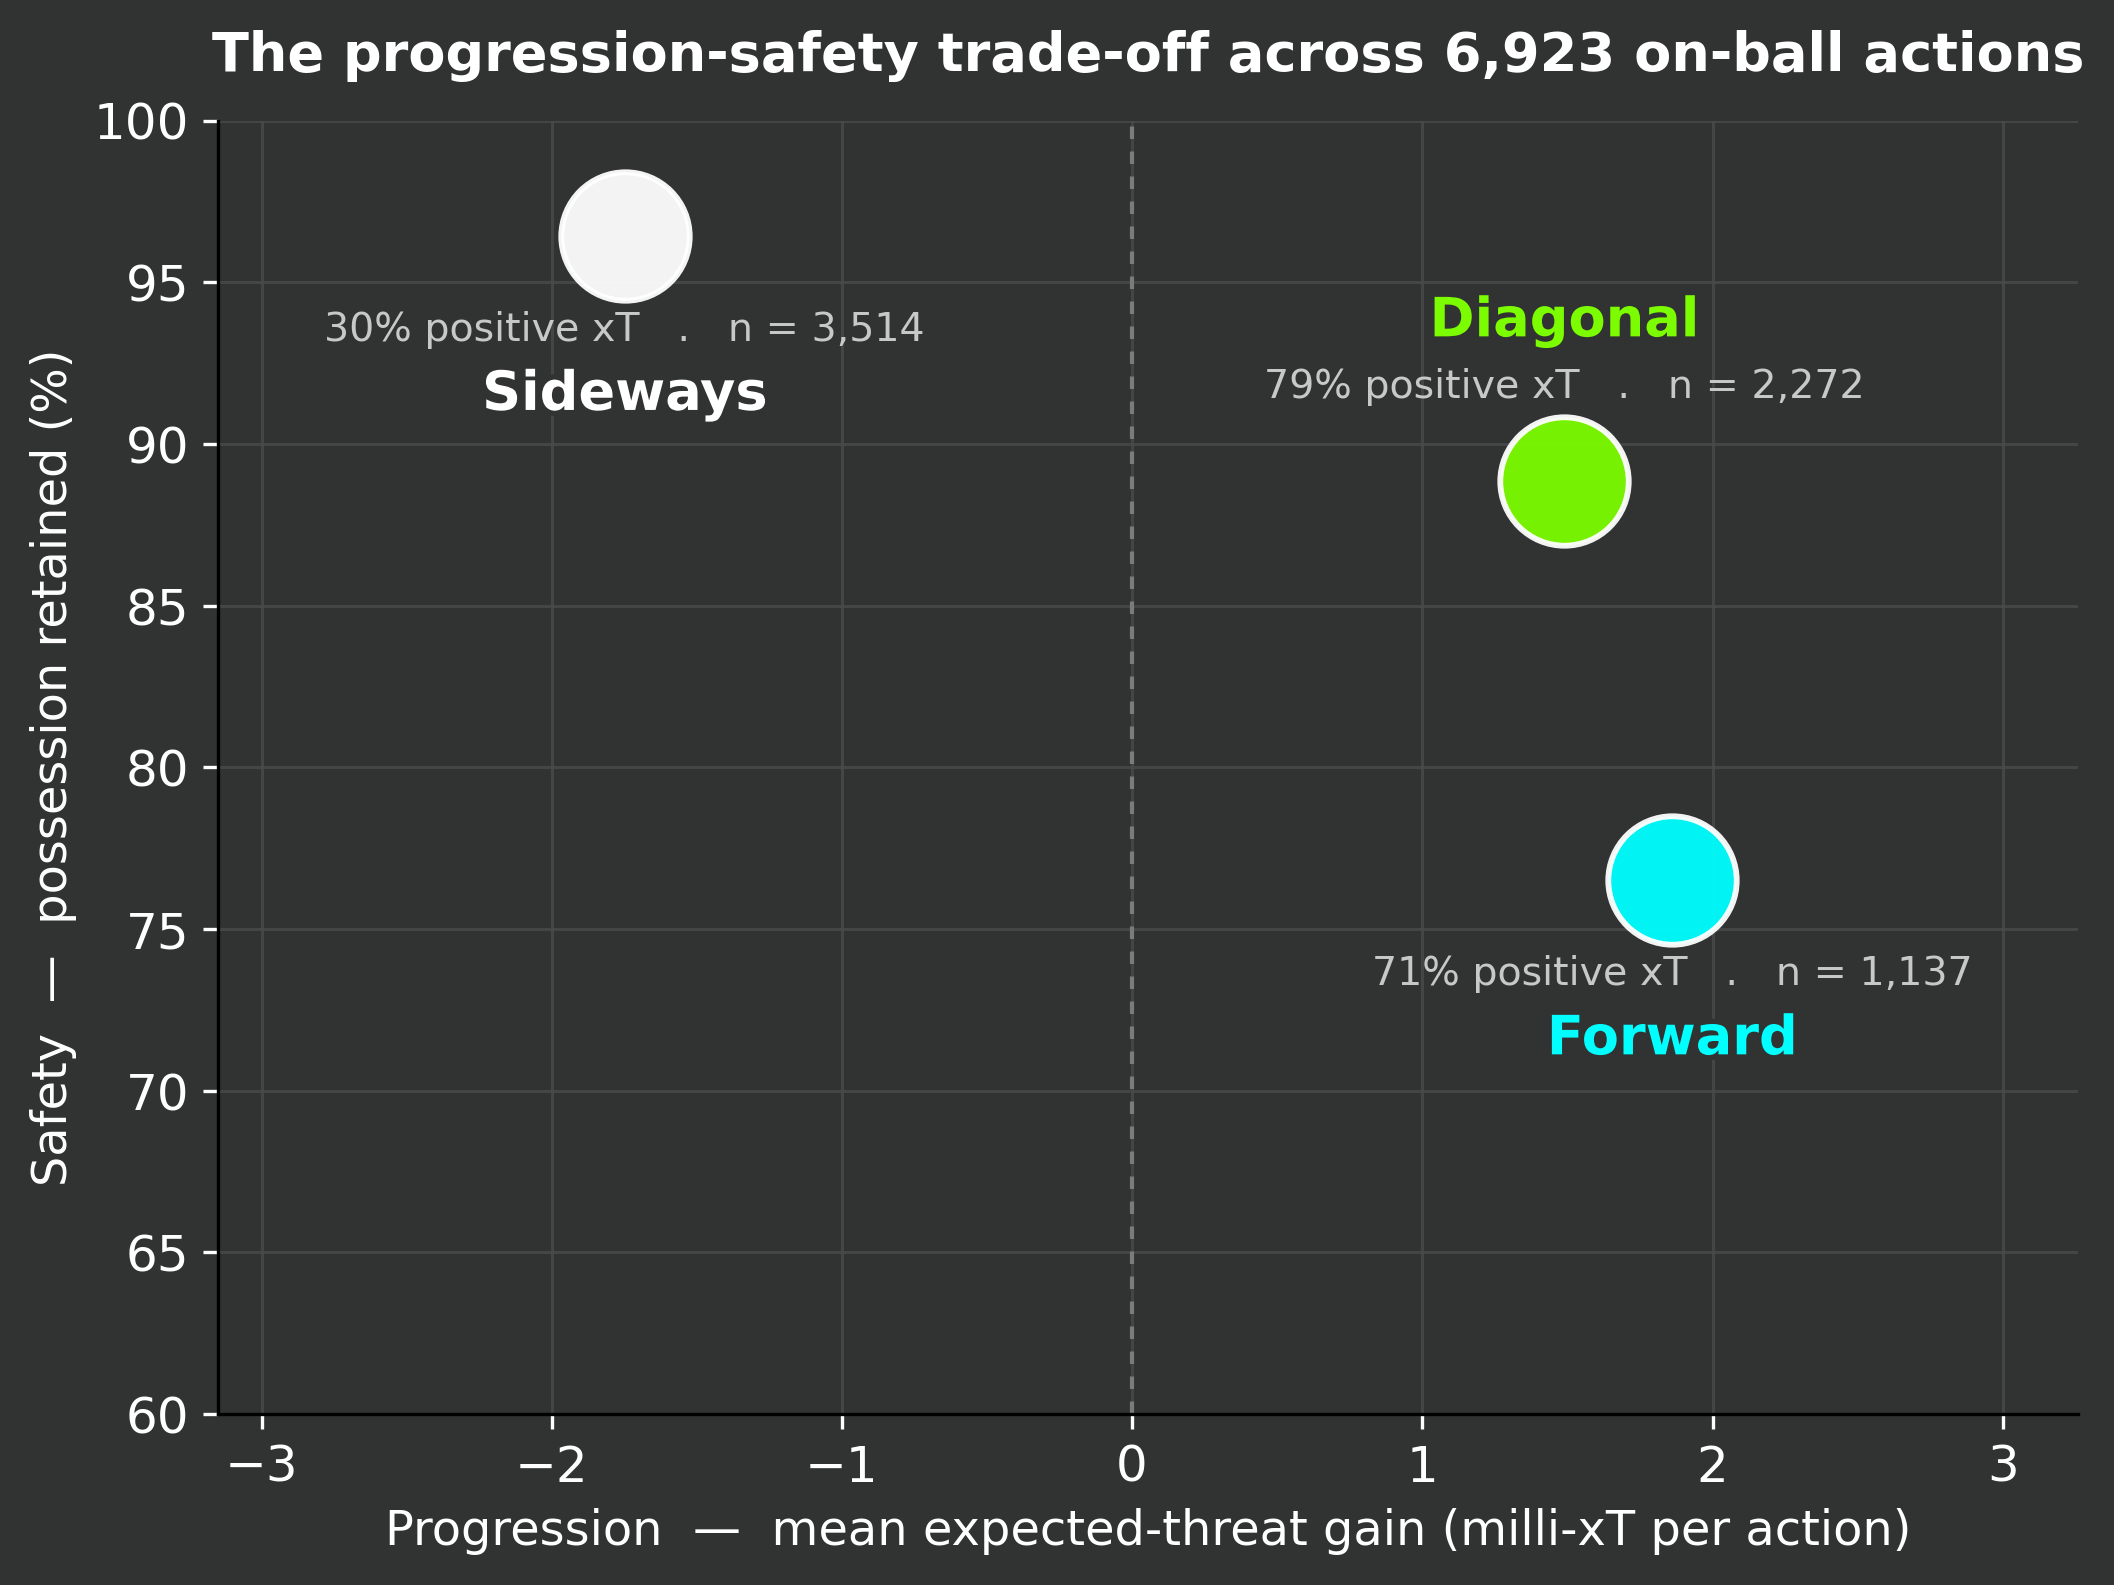
\includegraphics[width=0.74\textwidth]{Tradeoff.png}
  \caption{\textbf{The progression--safety trade-off across 6{,}923
  on-ball actions (H4).} Diagonal is not the extreme on either pole but
  the best joint outcome. Retention counts a completed pass, or possession
  kept through a carry or take-on.}
  \label{fig:tradeoff}
\end{figure}

\subsection{Bi-axial Disruption --- the Defender (H2)}
\label{sec:res-defender}

Why can the diagonal cheat the trade-off? On the defensive side,
Figure~\ref{fig:ddef} decomposes D-Def, three seconds after the action,
into its longitudinal (PC1) and lateral (PC2) components. Diagonal actions
are not the maximum of any single axis --- forward actions, which drive
straight at the block, disrupt PC1 as much. But the diagonal is the
\emph{lateral-disruption specialist}: its PC2 is significantly higher than
forward's ($p=7.0\times10^{-12}$), and its \emph{combined} PC1$+$PC2
disruption is the highest of the three classes ($p=2\times10^{-4}$).
\textbf{H2 holds}: a diagonal breaks the block on the very axis a vertical
pass leaves intact.

\begin{figure}[H]
  \centering
  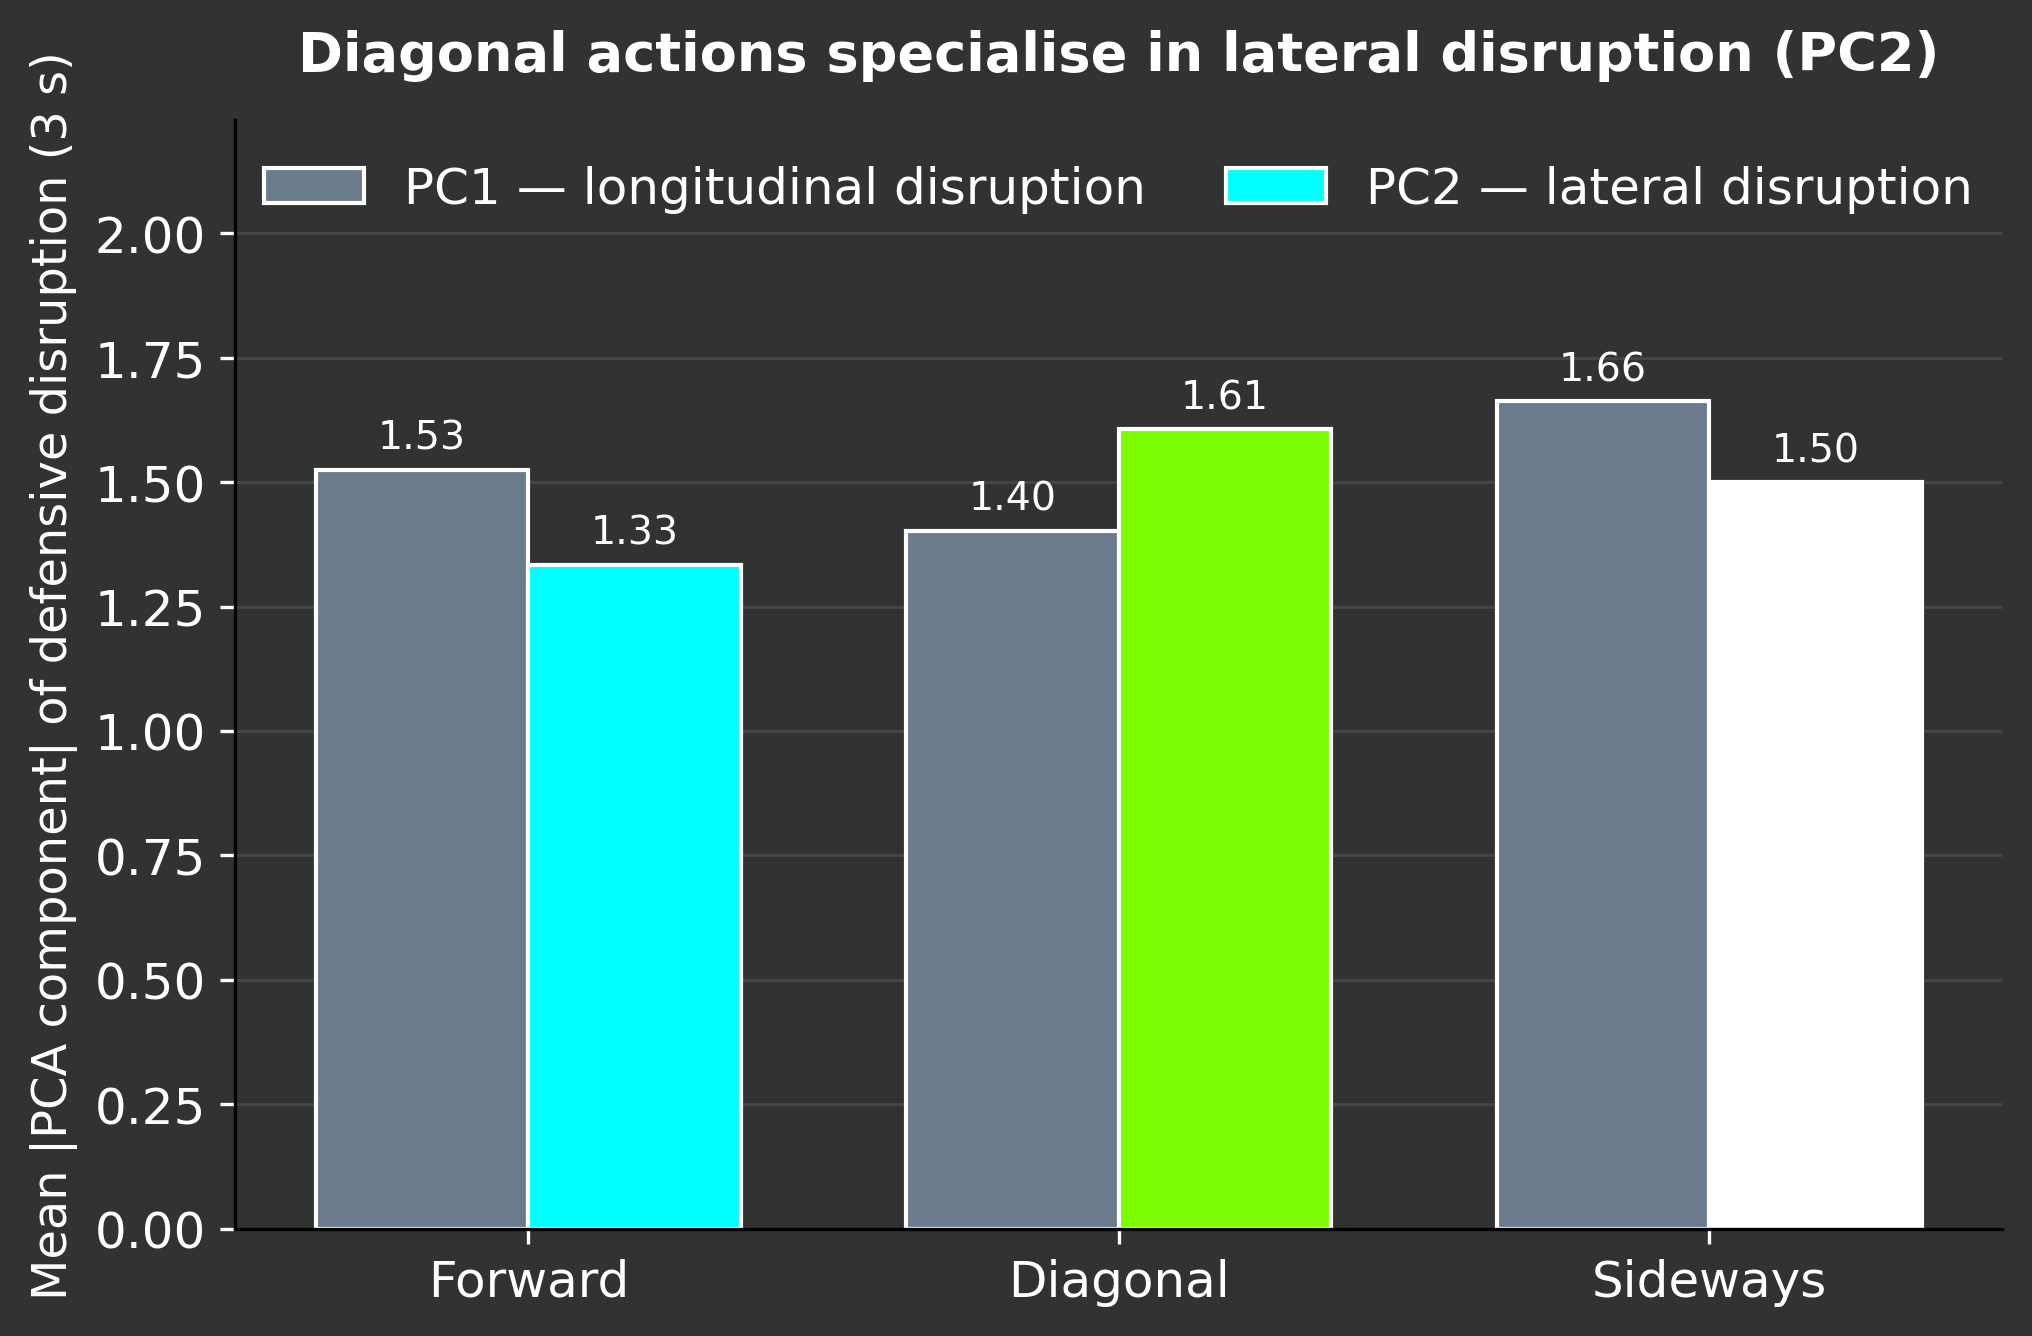
\includegraphics[width=0.66\textwidth]{DDef.png}
  \caption{\textbf{Defensive disruption (D-Def, Goes/Forcher; H2).}
  Per-event longitudinal (PC1) versus lateral (PC2) disruption three
  seconds after the action. Diagonal actions are the lateral-disruption
  specialists and carry the highest combined PC1$+$PC2 disruption.}
  \label{fig:ddef}
\end{figure}

\subsection{The Receiver's Advantage (H3)}
\label{sec:res-receiver}

On the attacking side, the advantage is one of perception
(Fig.~\ref{fig:receiver}). The receiver of a diagonal pass needs far less
rotation to face goal --- a mean head-to-goal angle of 108$^\circ$ against
145$^\circ$ for a forward pass ($p=1.6\times10^{-59}$, a large effect) ---
and has more team-mates inside the 120$^\circ$ binocular cone at the
moment of reception (6.0 against 5.0, $p=6.7\times10^{-11}$). The diagonal
receiver arrives, in Spielverlagerung's words, ``already in a position to
progress'', and in Hamilton's, at the point of maximum tactical
multiplicity \citep{hamilton2024}. \textbf{H3 holds.}

\begin{figure}[H]
  \centering
  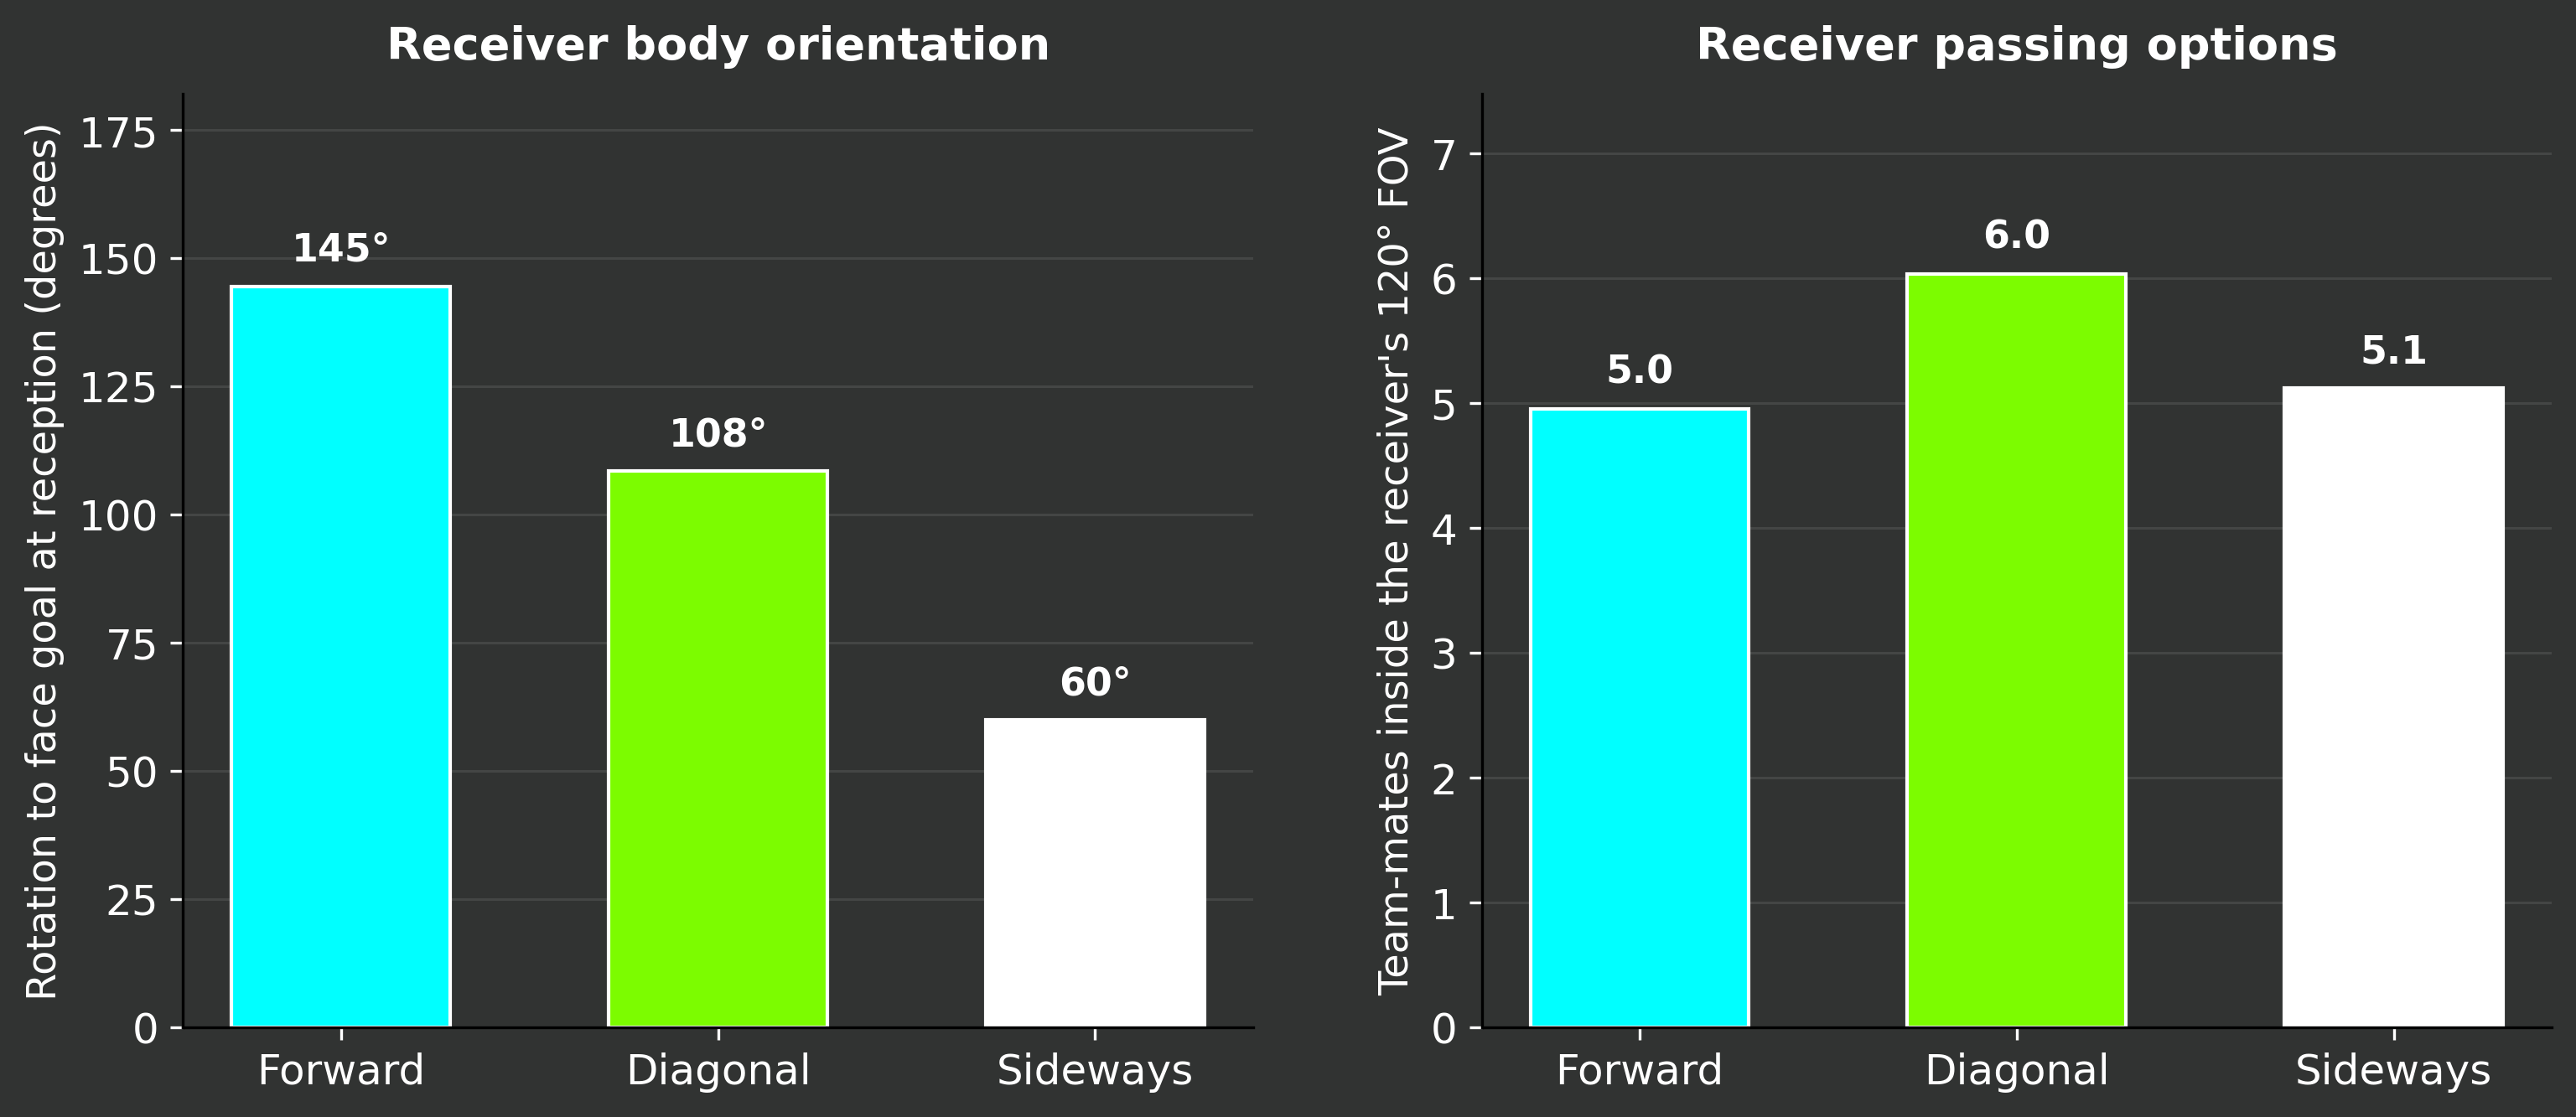
\includegraphics[width=0.92\textwidth]{Receiver.png}
  \caption{\textbf{Receiver advantage (H3).} The receiver of a diagonal
  pass needs far less rotation to face goal (left) and has more team-mates
  inside the 120$^\circ$ binocular cone at reception (right).}
  \label{fig:receiver}
\end{figure}

\paragraph{The article holds.} Diagonality is not folklore: on this
dataset it is Pareto-efficient, bi-axially disruptive, and kind to the
receiver. That settles \emph{whether} the diagonal works. It does not tell
a coach \emph{where} on the pitch, against \emph{which} defender, or a
player \emph{in the moment}. The rest of this paper answers that.

% =====================================================================
\section{The Diagonal Opportunity Surface}
\label{sec:dos}

The validation establishes that diagonal actions work; it does not locate
the opportunity. The Diagonal Opportunity Surface (DOS) does. DOS is a
real-time, \emph{action-independent} pitch map --- one routine scores a
pass, a carry, a take-on or an off-ball run --- that fuses three signals
into a single quantity of danger: what the on-ball player can \emph{see}
(Sec.~\ref{sec:vision}), what every player can physically \emph{reach}
(Sec.~\ref{sec:ppcf}), and how blind the defenders are to the threat
(Sec.~\ref{sec:dosdef}). A cognitive scanning gate (Sec.~\ref{sec:gate})
then restricts it to what the ball carrier can actually perceive, turning
a god-eye metric into a real-time decision tool.

\subsection{What the Player Sees --- the Vision Model}
\label{sec:vision}

For every player we build a probabilistic field of view, adapting the
model of \citet{bekkers2026} to TRACAB metres. The visible region is a
120$^\circ$ cone around the measured head yaw, with a Gaussian decay in
radial distance and in angular offset; both decays widen or narrow with
the player's speed, so a sprinting defender has a measurably tighter cone.
On top of the cone we compute occlusion: each other player casts an
angular shadow whose width is derived from that player's \emph{real}
shoulder width from the skeleton, plus a $12$\,cm anatomical correction
for soft tissue --- where \citet{bekkers2026} used a single fixed width
for everyone. The output is a per-player grid $V_i(x,y)\in[0,1]$: the
probability that player $i$ is visually aware of location $(x,y)$.

\begin{figure}[H]
  \centering
  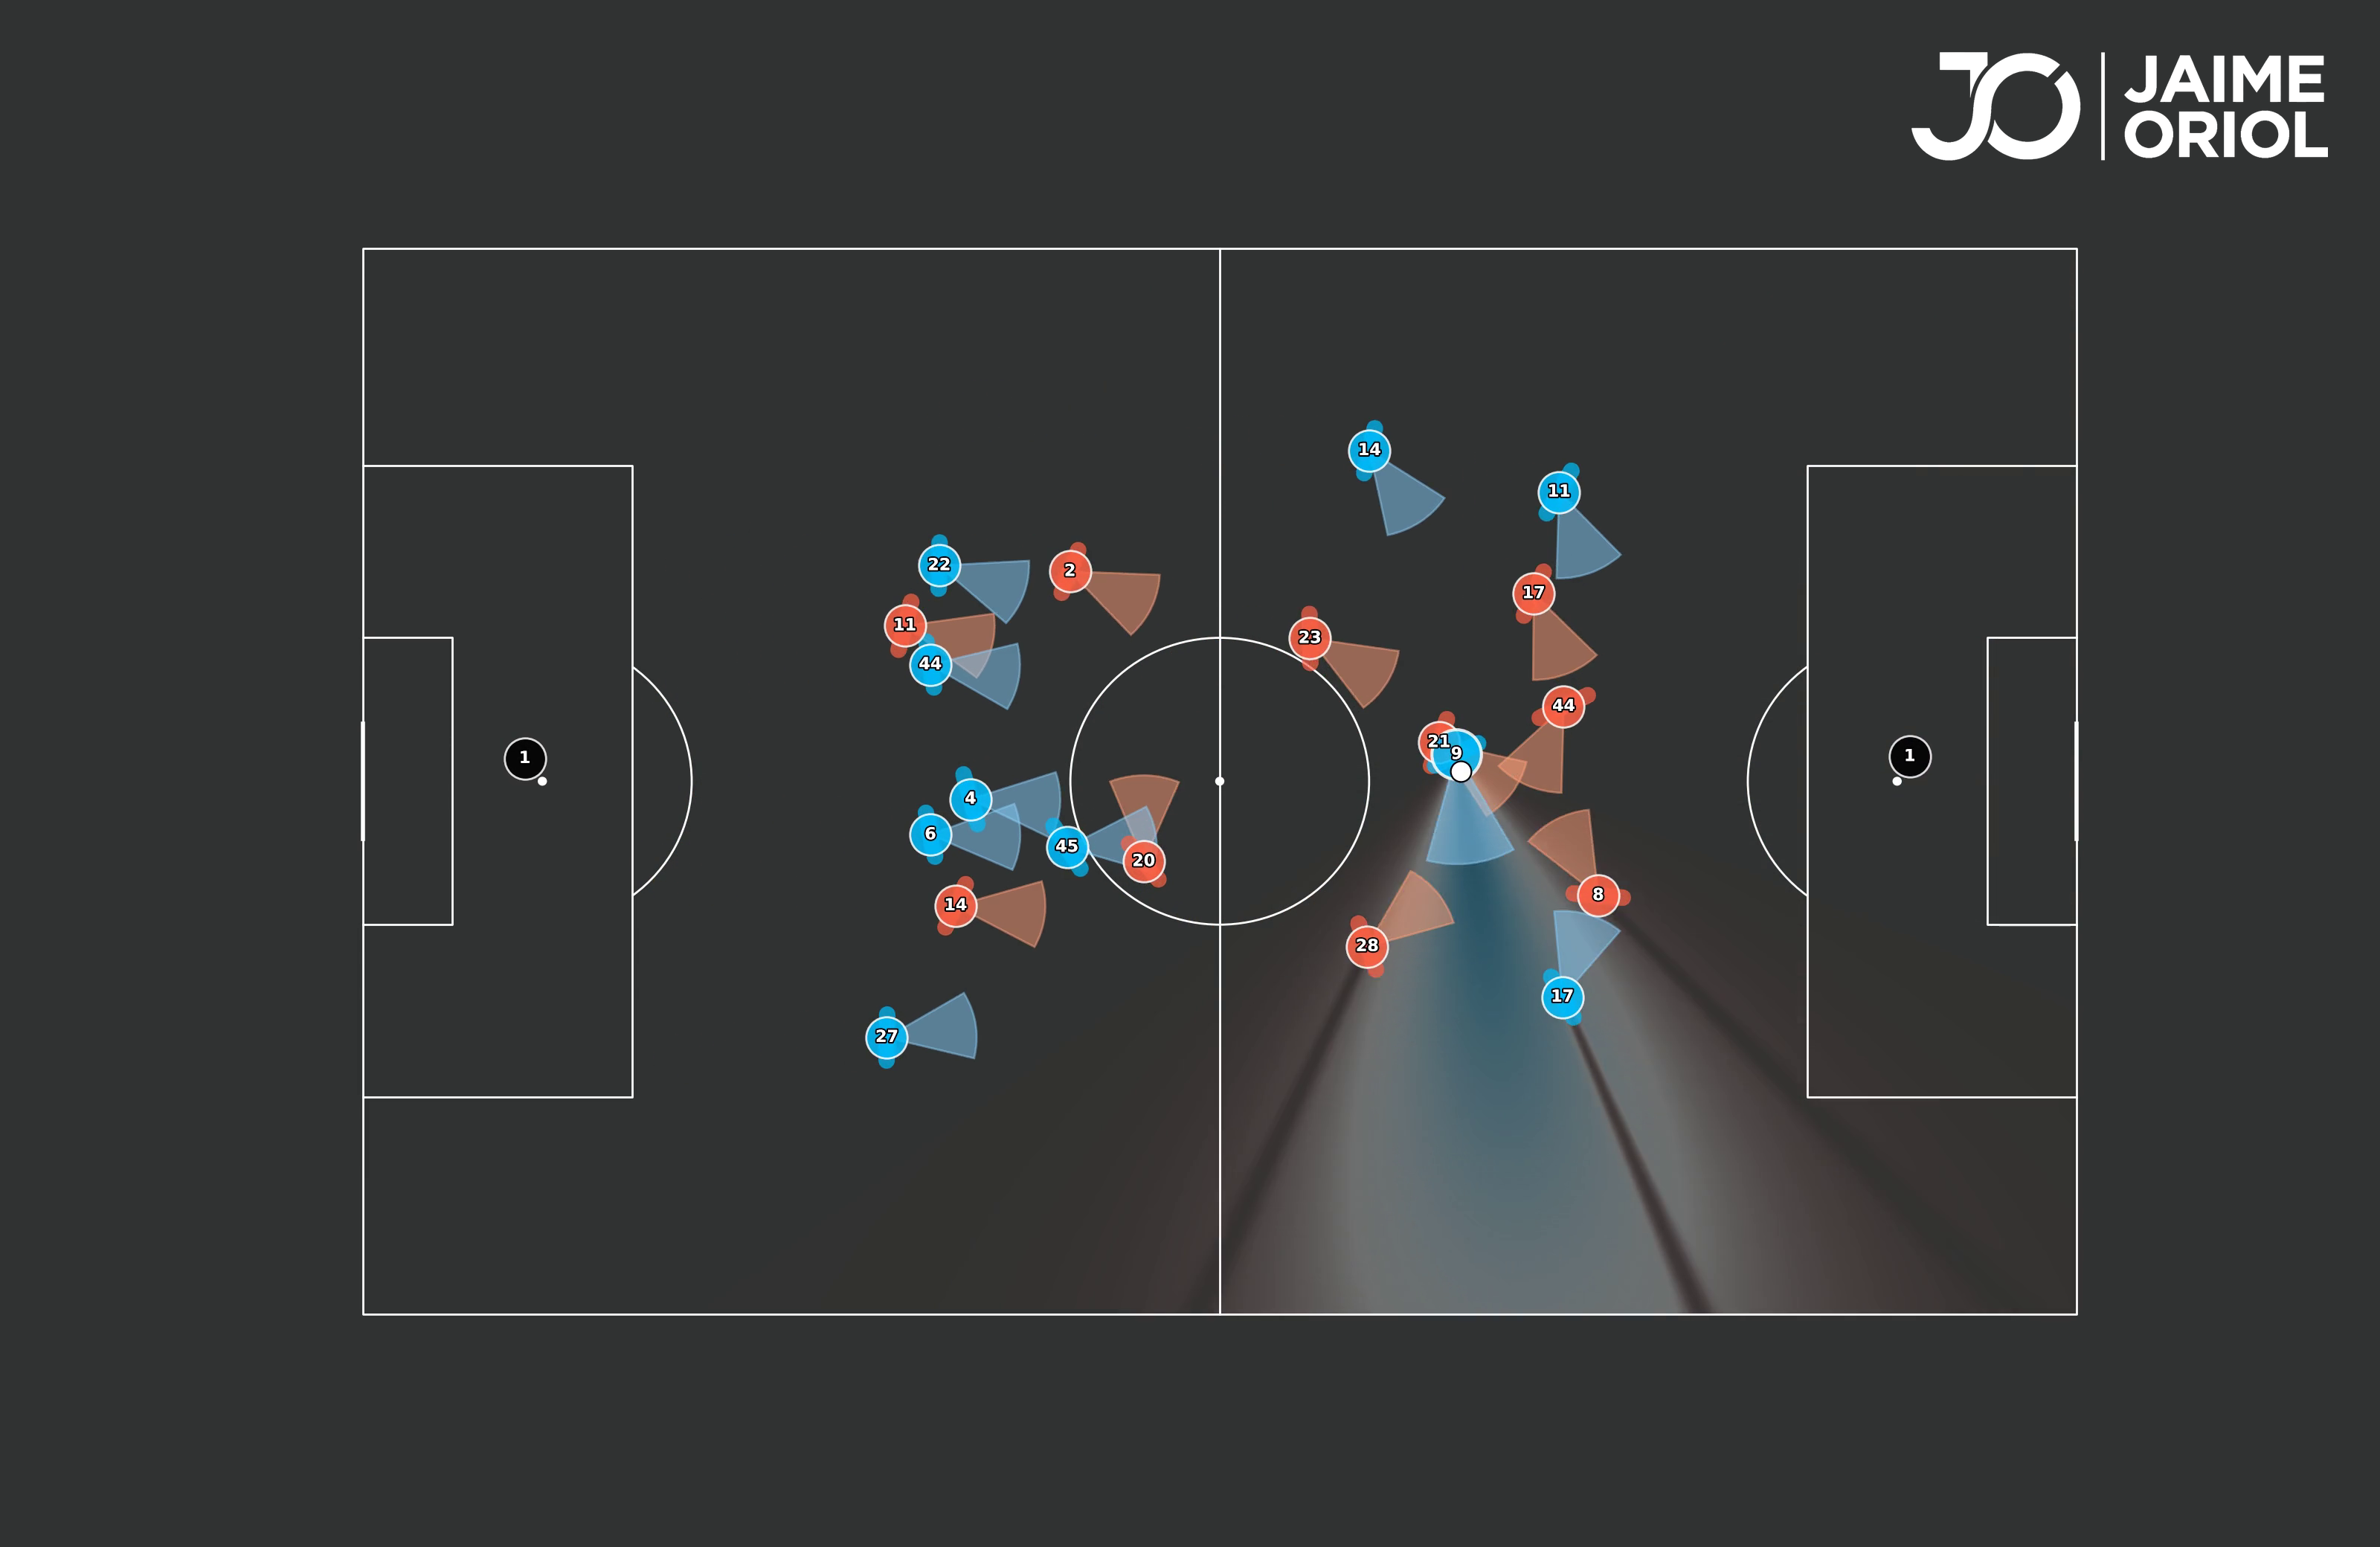
\includegraphics[width=\textwidth]{Vision.png}
  \caption{\textbf{Vision model.} Per-player field of view: a
  120$^\circ$ probabilistic cone with speed-dependent radial and angular
  decay, plus torso occlusion computed from the \emph{real} shoulder width
  of every occluder. Video:
  \videoref{figures/videos/Vision\_Video.mp4}{Vision\_Video.mp4}.}
  \label{fig:vision}
\end{figure}

\subsection{What the Player Can Reach --- Orientation-Aware Pitch Control}
\label{sec:ppcf}

Standard pitch control asks who reaches a cell first. We instead ask how
\emph{far} each player can usefully travel in an immediate window, given
that reacting to a stimulus behind them costs time. Each player is an
anisotropic Gaussian reach field. For player $i$ and target cell $x$, let
$\theta_i(x)$ be the unsigned angle between the player's measured shoulder
facing and the direction from the player to the cell. The
orientation-aware delay combines a reaction time and a change-of-direction
penalty:
\begin{align}
  \mathrm{rt}(\theta)  &= \mathrm{rt}_0
     + g\left(1+\exp\!\left[-\tfrac{\deg\theta - 60}{15}\right]\right)^{-1},
     &&\text{\citep{vater2024}}\\
  \mathrm{cod}(\theta) &= A\,\sin^2(\theta/2), &&\text{\citep{dossantos2018}}\\
  \mathrm{delay}_i(x)  &= \mathrm{rt}(\theta_i(x)) + \mathrm{cod}(\theta_i(x)).
\end{align}
Here $\mathrm{rt}_0$ is the base reaction time and $g$ its
orientation-dependent gain. During the delay the
player drifts at current velocity, $\mathrm{drift}_i(x) = \mathrm{pos}_i +
\mathrm{vel}_i\cdot\mathrm{delay}_i(x)$, and the remaining travel budget is
$\mathrm{reach}_i(x) = \max(0,\,W-\mathrm{delay}_i(x))\cdot v_{\max}$ for an
integration window $W$. The reach modulates the width of the player's
influence Gaussian,
\begin{equation}
  \sigma_i(x) = \sigma_0\left[(1-m) + m\,\frac{\mathrm{reach}_i(x)}{\mathrm{reach}_{\max}}\right],
  \qquad
  \mathrm{infl}_i(x) = \exp\!\left(-\frac{\lVert x-\mathrm{drift}_i(x)\rVert^2}{2\,\sigma_i(x)^2}\right).
\end{equation}
A defender facing a cell keeps a full-width blob; a defender with that
cell in their blind spot has a blob compressed to half-width --- a literal
hole in their control field. Per-team influences are summed,
$I_\mathrm{att} = \sum_{i\in\mathrm{att}}\mathrm{infl}_i$ and
$I_\mathrm{def}$ likewise, and converted to control shares:
\begin{equation}
  \mathrm{ppcf}_\mathrm{att} =
  \left(1-e^{-(I_\mathrm{att}+I_\mathrm{def})}\right)
  \frac{I_\mathrm{att}}{I_\mathrm{att}+I_\mathrm{def}}.
\end{equation}

\begin{figure}[H]
  \centering
  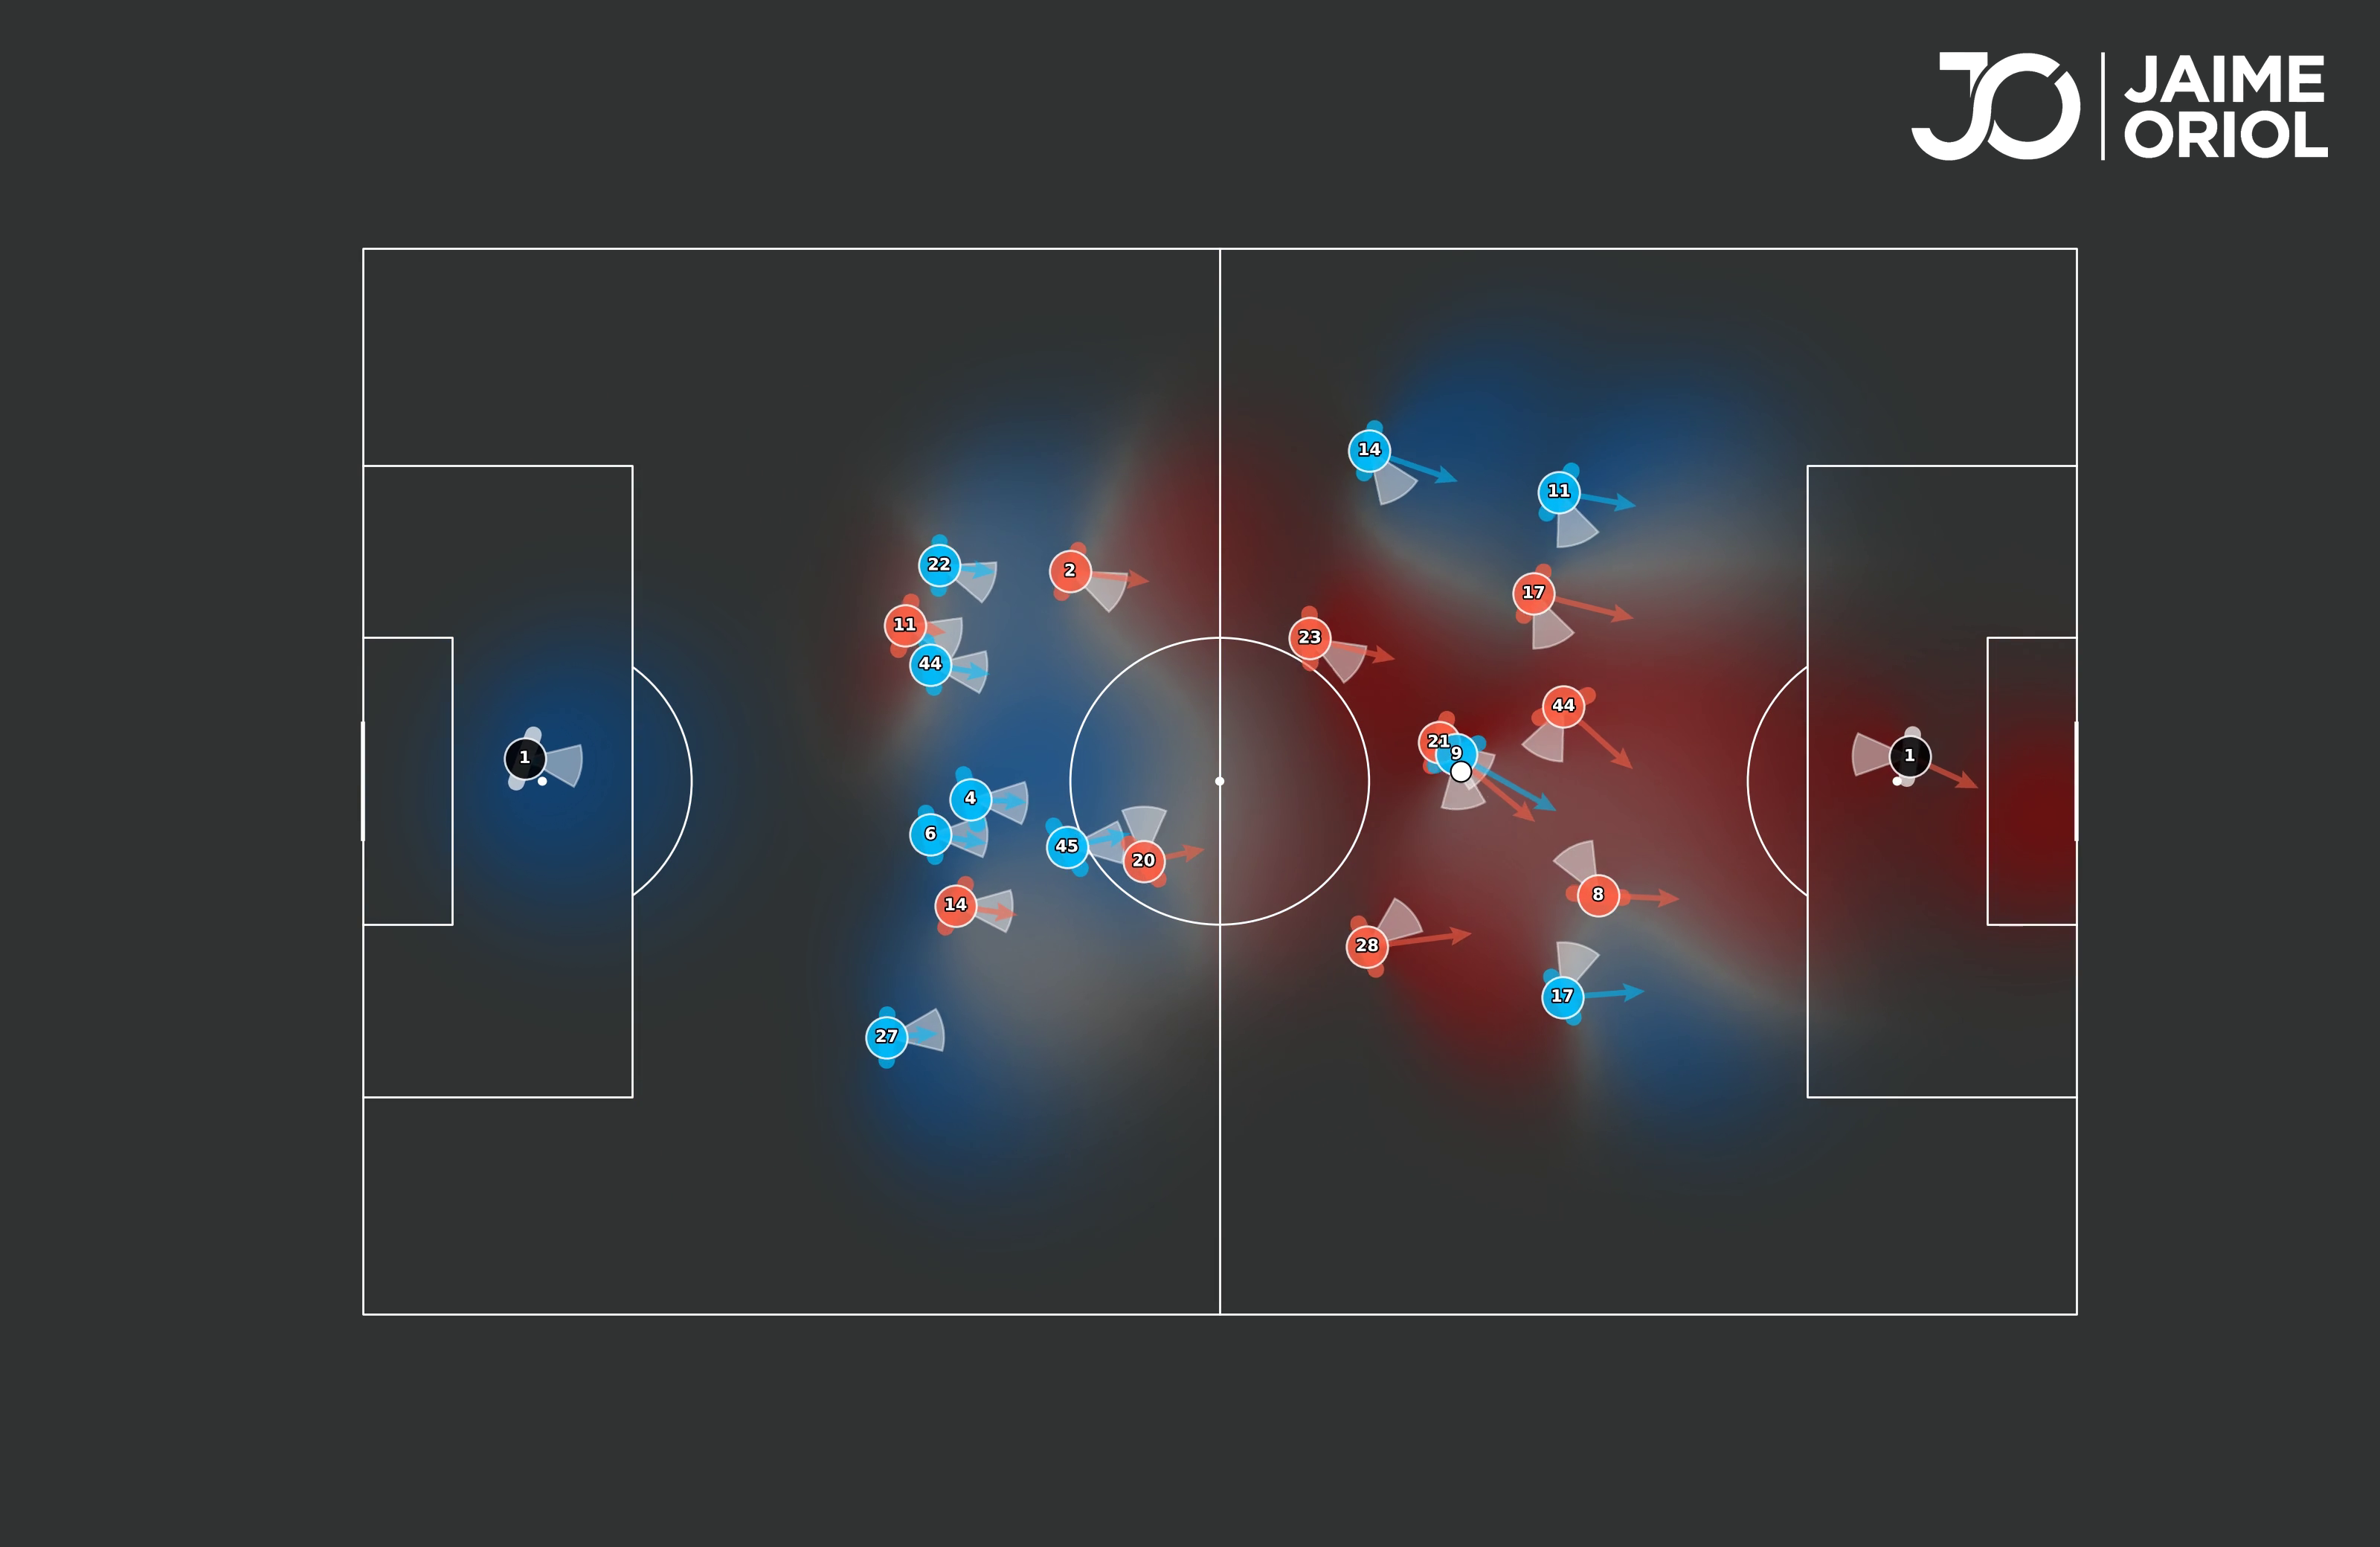
\includegraphics[width=\textwidth]{PPCF.png}
  \caption{\textbf{Orientation-Aware Pitch Control.} Each player is an
  anisotropic reach field whose width follows the orientation-aware
  reaction delay (Vater reaction time + Dos'Santos change-of-direction
  penalty applied to the real shoulder angle). A defender with the threat
  in his blind spot has a visible hole in his control field. Video:
  \videoref{figures/videos/PPCF\_Video.mp4}{PPCF\_Video.mp4}.}
  \label{fig:ppcf}
\end{figure}

\subsection{The Surface --- Danger from a Blind Defender}
\label{sec:dosdef}

DOS measures, for every cell, how much extra control the attacking team
buys by delivering the ball diagonally rather than straight:
\begin{equation}
  \mathrm{DOS}(x,y) = \max_{d\,\in\,\text{diag}}\mathrm{ppcf}_\mathrm{att}^{(d)}(x,y)
                    - \max_{d\,\in\,\text{fwd}}\mathrm{ppcf}_\mathrm{att}^{(d)}(x,y).
\end{equation}
The mechanism is H1 made computable. A defender who cannot see the threat
reacts late, and that late reaction shrinks their reach blob. For each
defender we score awareness from two vision signals --- can they see the
attacker, and can they see the ball ---
\begin{equation}
  \mathrm{awareness}_i = \mathrm{clip}\big[(0.7\,V_i^\mathrm{att} + 0.3\,V_i^\mathrm{ball})
     \cdot p_\mathrm{speed}\cdot p_\mathrm{diag},\;0,\,1\big],
\end{equation}
where $p_\mathrm{speed}$ and $p_\mathrm{diag}$ are small penalties for fast
and oblique attackers (the brain misjudges oblique closing speed). Low
awareness injects an extra detection delay,
$\mathrm{delay}^{\mathrm{det}}_i = \max(0,\,(\mathrm{rt}(\theta^\mathrm{threat}_i)
- \mathrm{rt}_0)\,(1-\mathrm{awareness}_i))$, which feeds back into the
reach field of Sec.~\ref{sec:ppcf}. Where defenders are blind their blobs
collapse and DOS lights up. A high-DOS cell is therefore the sum of three
readable ingredients: a defender \emph{blind spot}, an \emph{orientation
delay} in reaching it, and the \emph{directional benefit} of arriving
oblique. Because DOS only needs an origin and a direction, the same
routine scores any action --- pass, carry, take-on or off-ball run.

\begin{figure}[H]
  \centering
  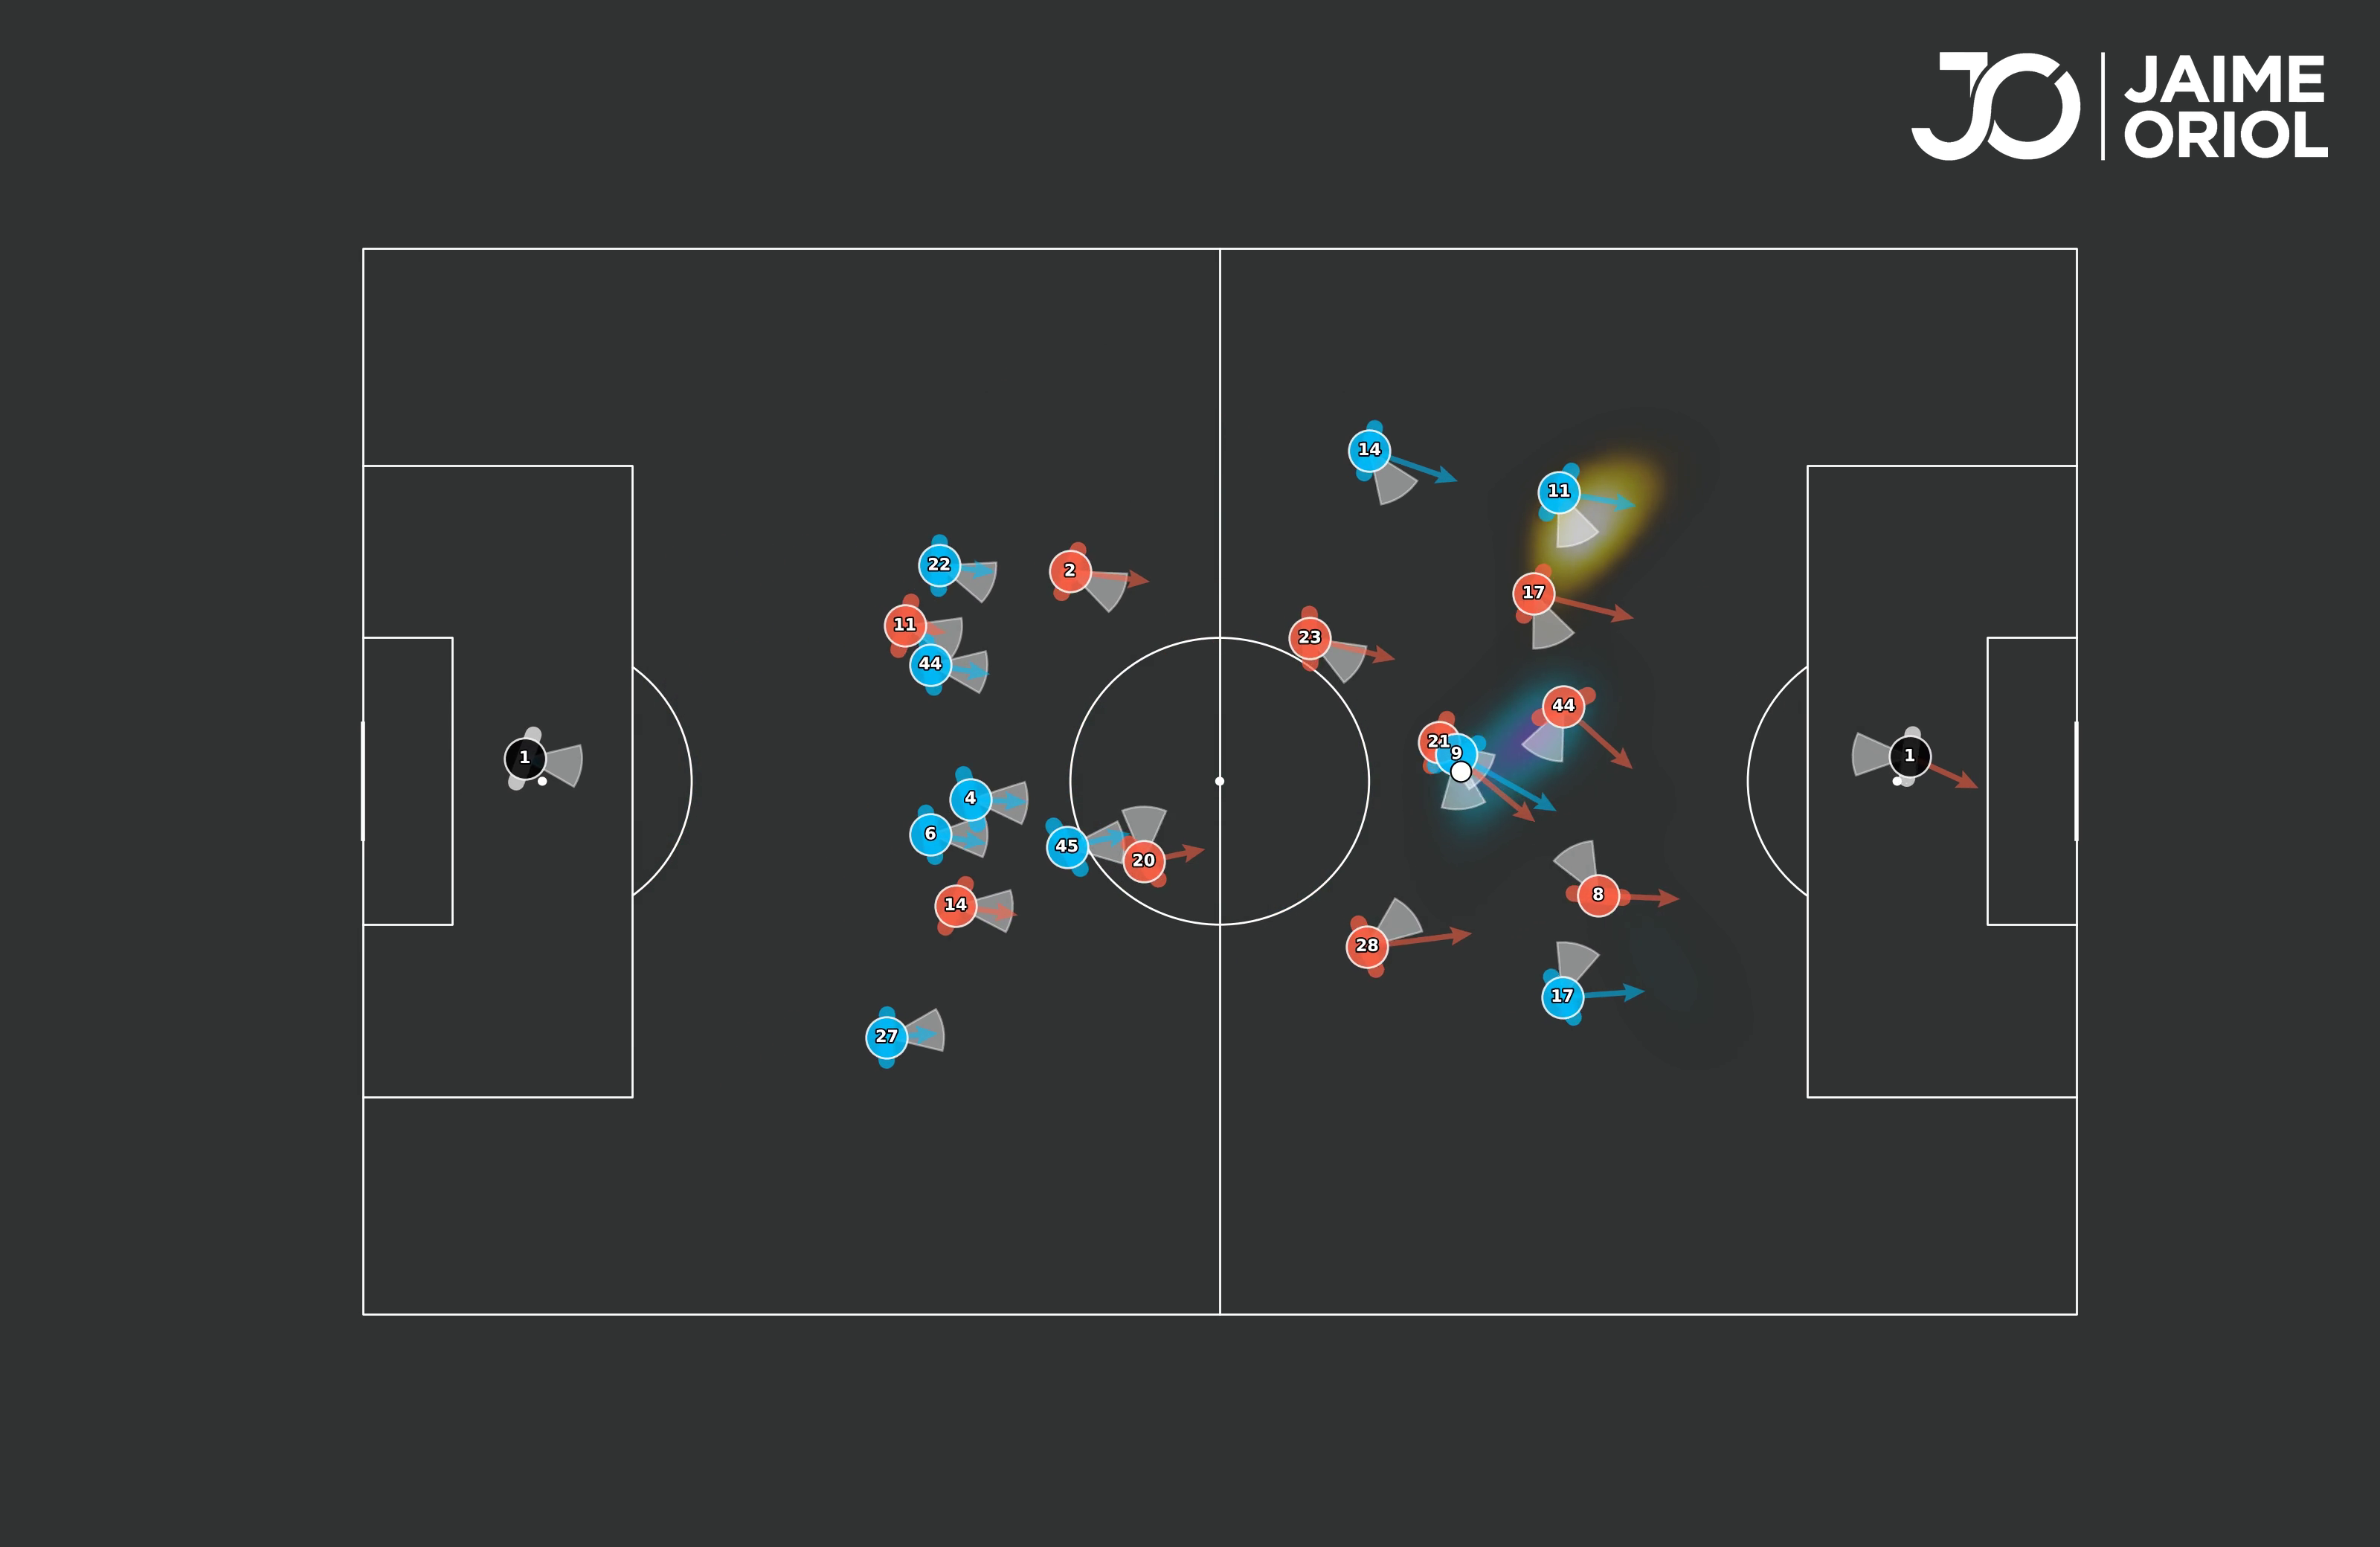
\includegraphics[width=\textwidth]{DOS.png}
  \caption{\textbf{Diagonal Opportunity Surface.} For every cell, DOS is
  the extra attacker pitch control bought by the best diagonal delivery
  over the best orthogonal one, given the defenders' real orientation and
  what they can see. Video:
  \videoref{figures/videos/DOS\_Video.mp4}{DOS\_Video.mp4}.}
  \label{fig:dos}
\end{figure}

\subsection{The Real-Time Engine --- the Cognitive Scanning Gate}
\label{sec:gate}

A god-eye DOS surface is not actionable: a player cannot exploit an
opportunity they cannot perceive. We therefore gate DOS by what the
on-ball player actually sees. A frame-exact possession timeline ---
carries and passes linked to their receptions through the
\texttt{play\_id} field --- identifies the on-ball owner at every frame.
For that owner we compute a scanning memory: the maximum, over the last
2.5\,s, of their own field of view weighted by an exponential recency
decay ($\tau=1.2$\,s). The lookback grows linearly from zero at the moment
a player becomes on-ball, so a receiver never inherits the passer's
pre-pass scan; on a pass the gate transitions cleanly to the receiver's
field of view. Only cells the owner can see, or has recently scanned, are
painted. The result is a real-time, perception-bounded reading: at every
frame it shows which \textbf{passes} (inside the field of view),
\textbf{dribbles} (off the defender's mis-orientation) and \textbf{runs}
the player can both \emph{see} and \emph{reach}, and where the danger ---
high DOS --- lies. A second, ``shadow'' layer marks high-DOS cells the
player does \emph{not} see but that lie ahead in realistic range ---
Hamilton's \emph{shadowpass} \citep{hamilton2024}.

\subsection{DOS Predicts Value}
\label{sec:res-dos}

DOS is validated against expected-threat delta $\Delta\mathrm{xT}$
\citep{singh2018}, an outcome it never sees: the DOS model receives no xG,
no xT and no success labels, only geometry, the vision model and skeleton
orientation, so DOS and $\Delta\mathrm{xT}$ are mathematically
independent. Across all actions, events that gain expected threat carry
significantly higher DOS (Mann--Whitney $U$, $p=1.16\times10^{-25}$); the
effect is strongest for carries (rank-biserial correlation $+0.40$,
$p=1.2\times10^{-36}$), whose multi-frame trajectory is exactly where a
diagonal moment can be isolated. Sorting actions into DOS quintiles
(Fig.~\ref{fig:quintiles}), the rate of positive expected-threat outcomes
rises monotonically from 43\% to 61\%. The relationship survives a
logistic regression that controls for pass distance, pressure on the
passer and the number of defenders in the lane and goal-side (DOS
coefficient $+10.9$, $p=2.6\times10^{-5}$). DOS captures something beyond
geometry, pressure and defender counts.

\begin{figure}[H]
  \centering
  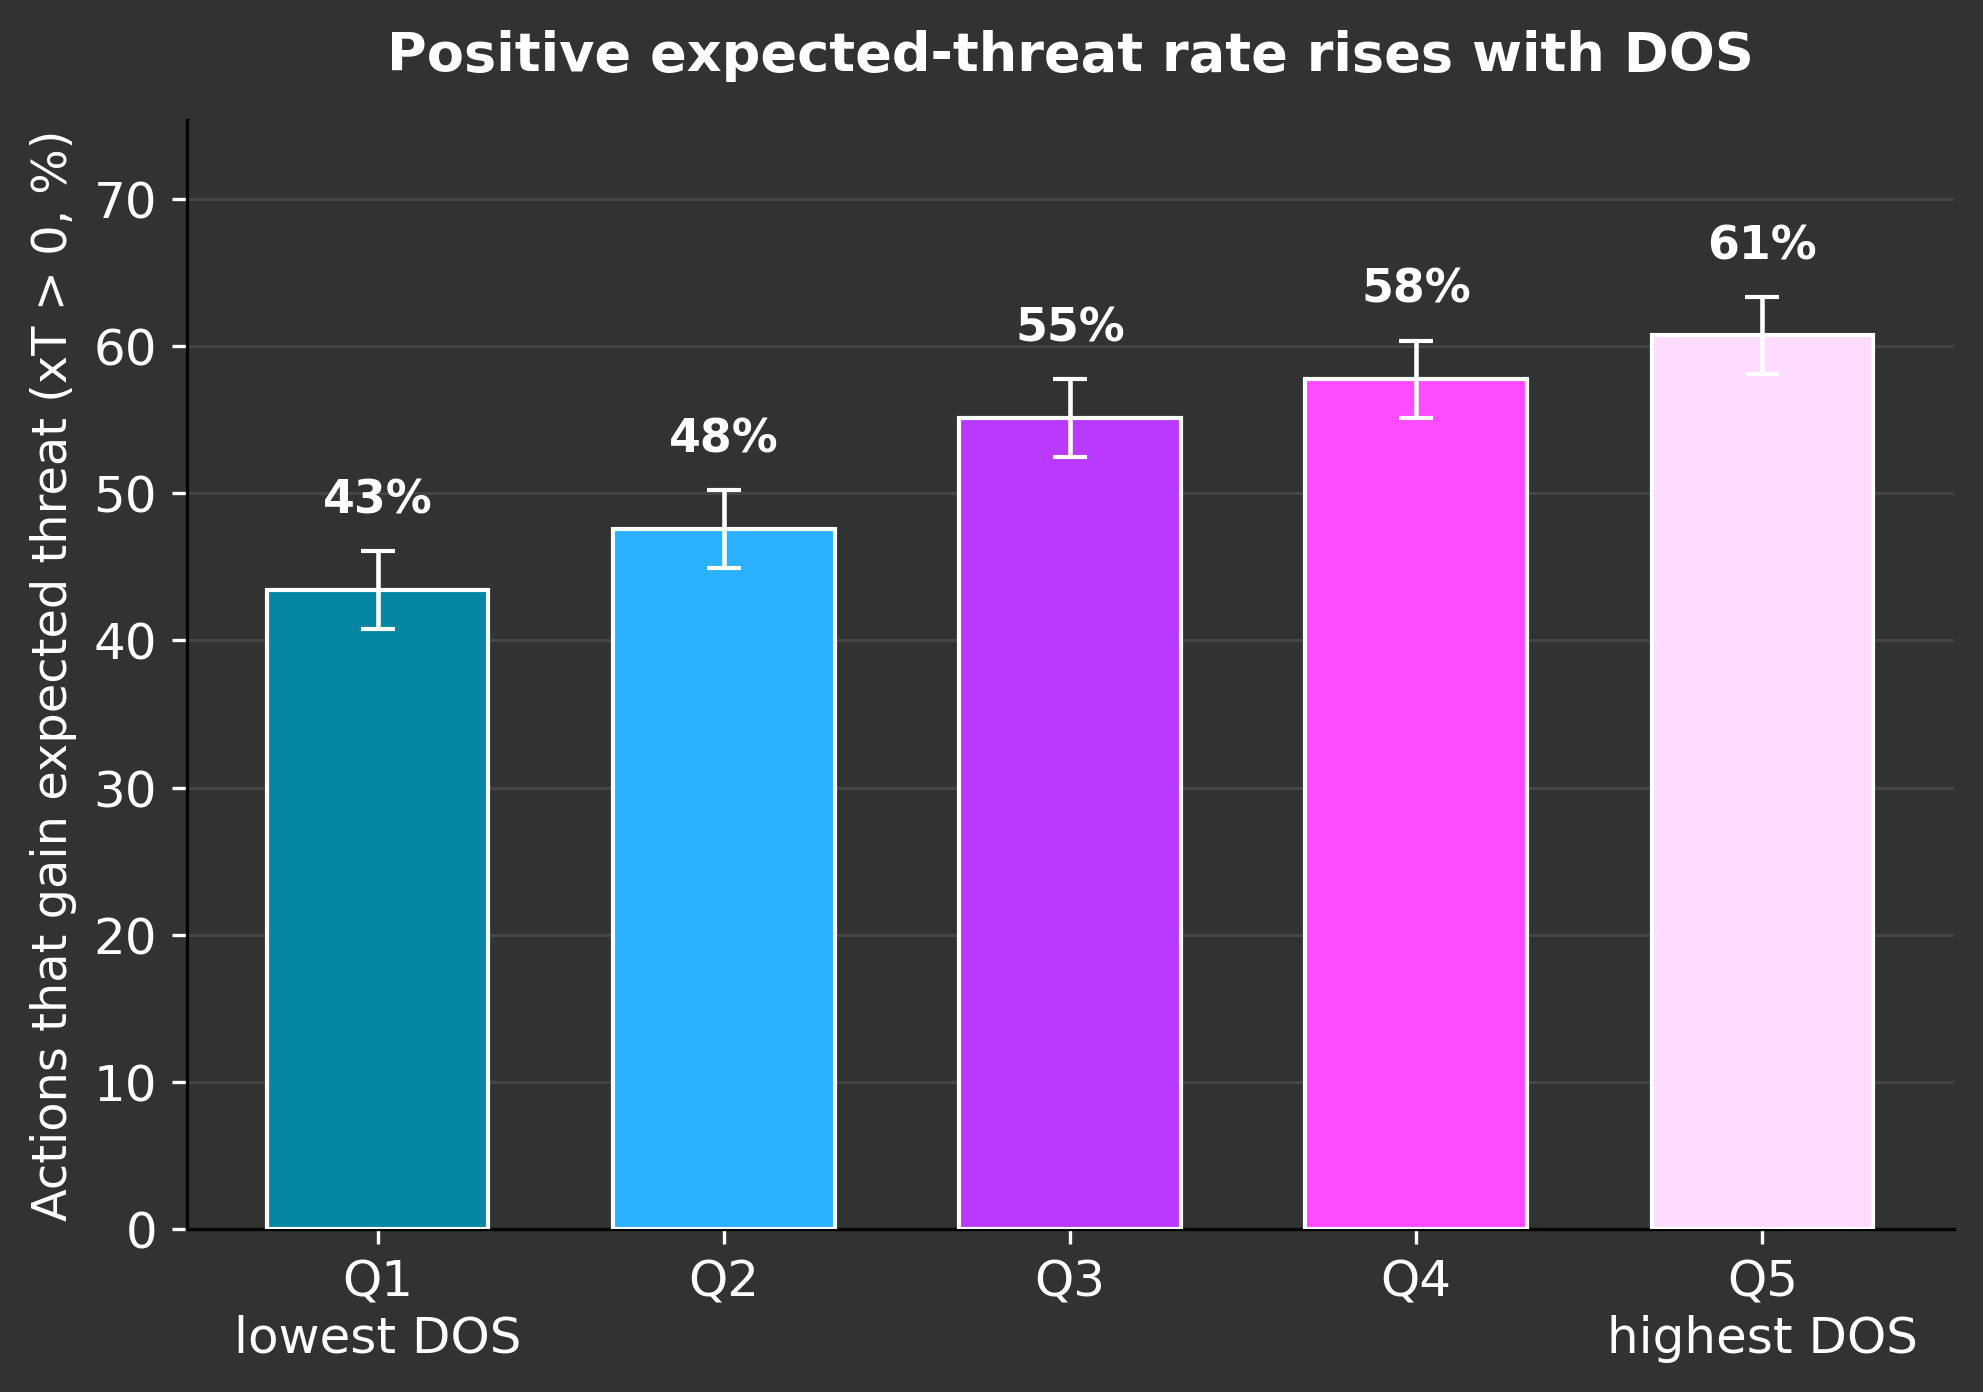
\includegraphics[width=0.66\textwidth]{Quintiles.png}
  \caption{\textbf{DOS predicts value.} Across DOS quintiles the rate of
  positive expected-threat outcomes rises monotonically. DOS and expected
  threat are mathematically independent --- the model sees no xG, no xT
  and no outcome labels.}
  \label{fig:quintiles}
\end{figure}

\subsection{The Third Action --- Off-Ball Runs}
\label{sec:runs}

Because DOS is action-independent, off-ball runs --- the third way to
progress --- pass through the same routine as passes and carries. Run
\emph{detection} is a mature commercial front-end: SkillCorner Game
Intelligence \citep{skillcorner2024} and Opta Vision \citep{optavision2025}
both detect and classify runs, and \citet{llana2022} value them. We do not
re-derive a run taxonomy; we use a lightweight detector aligned to that
public notion --- an attacking player who is not the ball carrier,
sustaining above $5$\,m/s for at least $0.7$\,s with a net displacement
above $5$\,m --- and score each detected run with DOS exactly as a
take-on is. This yields 2{,}354 runs, physically
coherent (a mean duration of 2.8\,s, 16.8\,m of displacement, a 6.4\,m/s
peak), of which 89.8\% carry positive DOS: off-ball movement, like on-ball
action, is mostly a search for the defender's blind side. Our contribution
is not the detection but the orientation-aware valuation that any such
front-end can feed.

\subsection{The Coaching Deliverable}
\label{sec:res-map}

Aggregated over all actions and binned by pitch zone,
Figure~\ref{fig:dosmap} is the framework's coach-facing output: a map of
where diagonal play pays off. DOS rises smoothly toward the attacking goal
and is highest in the zones flanking the box --- the half-spaces
Spielverlagerung identifies as ``the ideal intersection of \emph{I have
enough space} and \emph{what I can't see doesn't matter}''. Aggregated per
opponent rather than over the whole sample, the same map becomes a
scouting tool: a picture of where a specific team's defenders habitually
orient away from danger. As a case study, Figure~\ref{fig:olise} profiles
a single player's passing through the diagonality lens --- a direct
scouting output of the framework.

\begin{figure}[H]
  \centering
  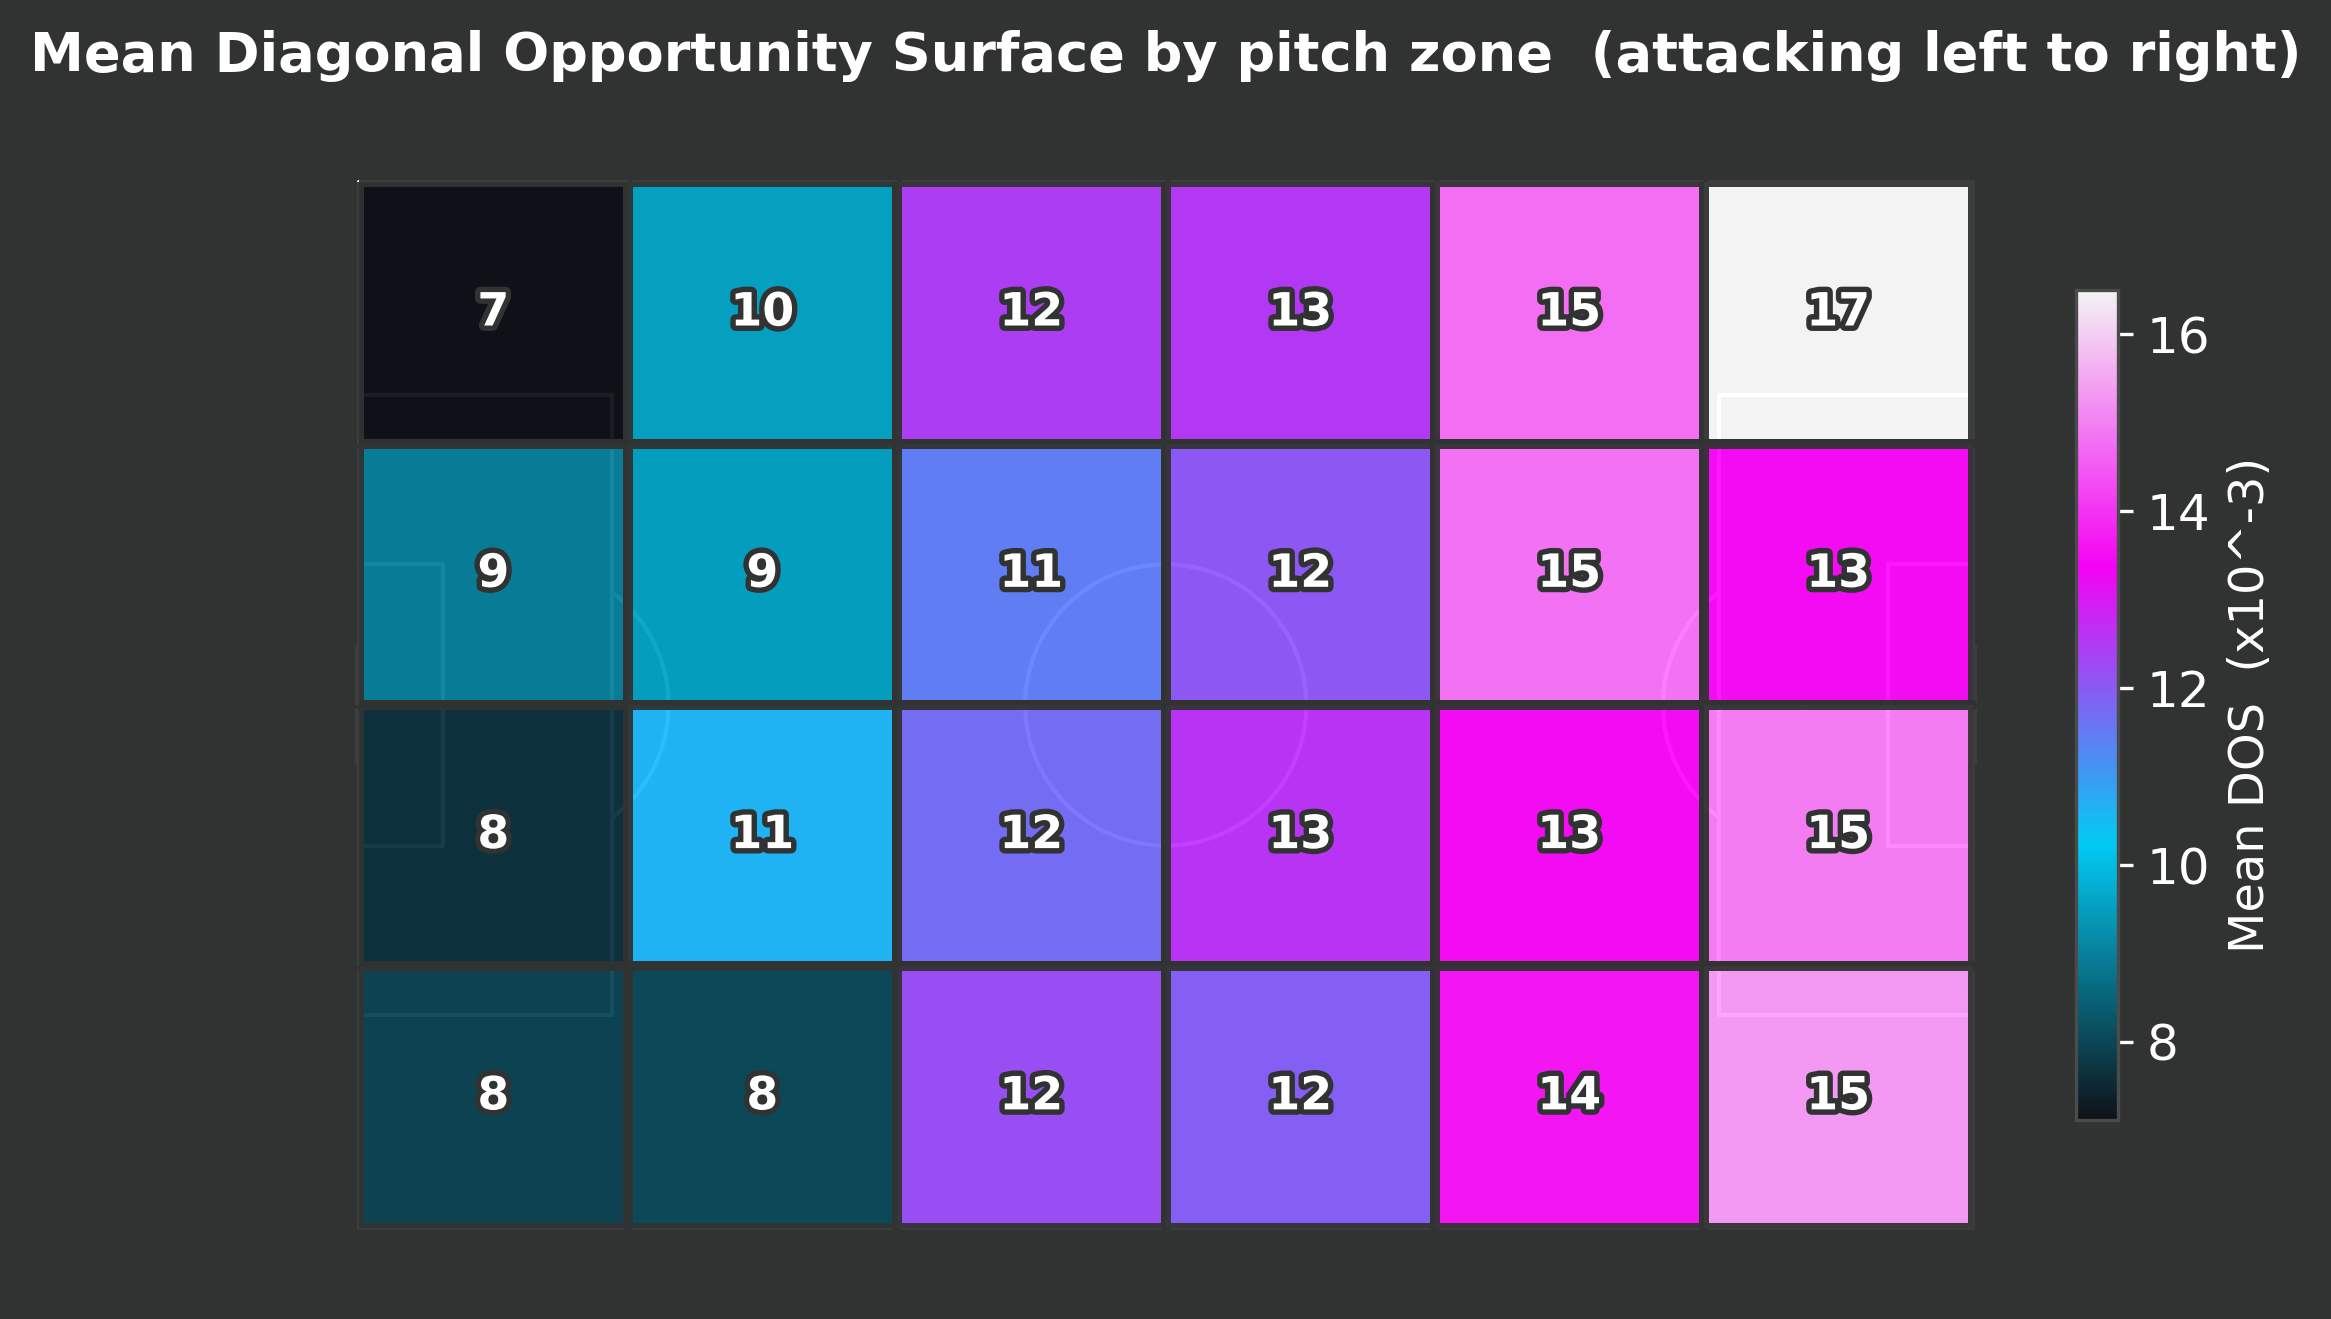
\includegraphics[width=0.80\textwidth]{DOS_Map.png}
  \caption{\textbf{Where diagonal play pays off.} Mean DOS by pitch zone
  over 6{,}923 actions, every attack normalised left to right. DOS rises
  toward the attacking goal and peaks in the half-spaces.}
  \label{fig:dosmap}
\end{figure}

\begin{figure}[H]
  \centering
  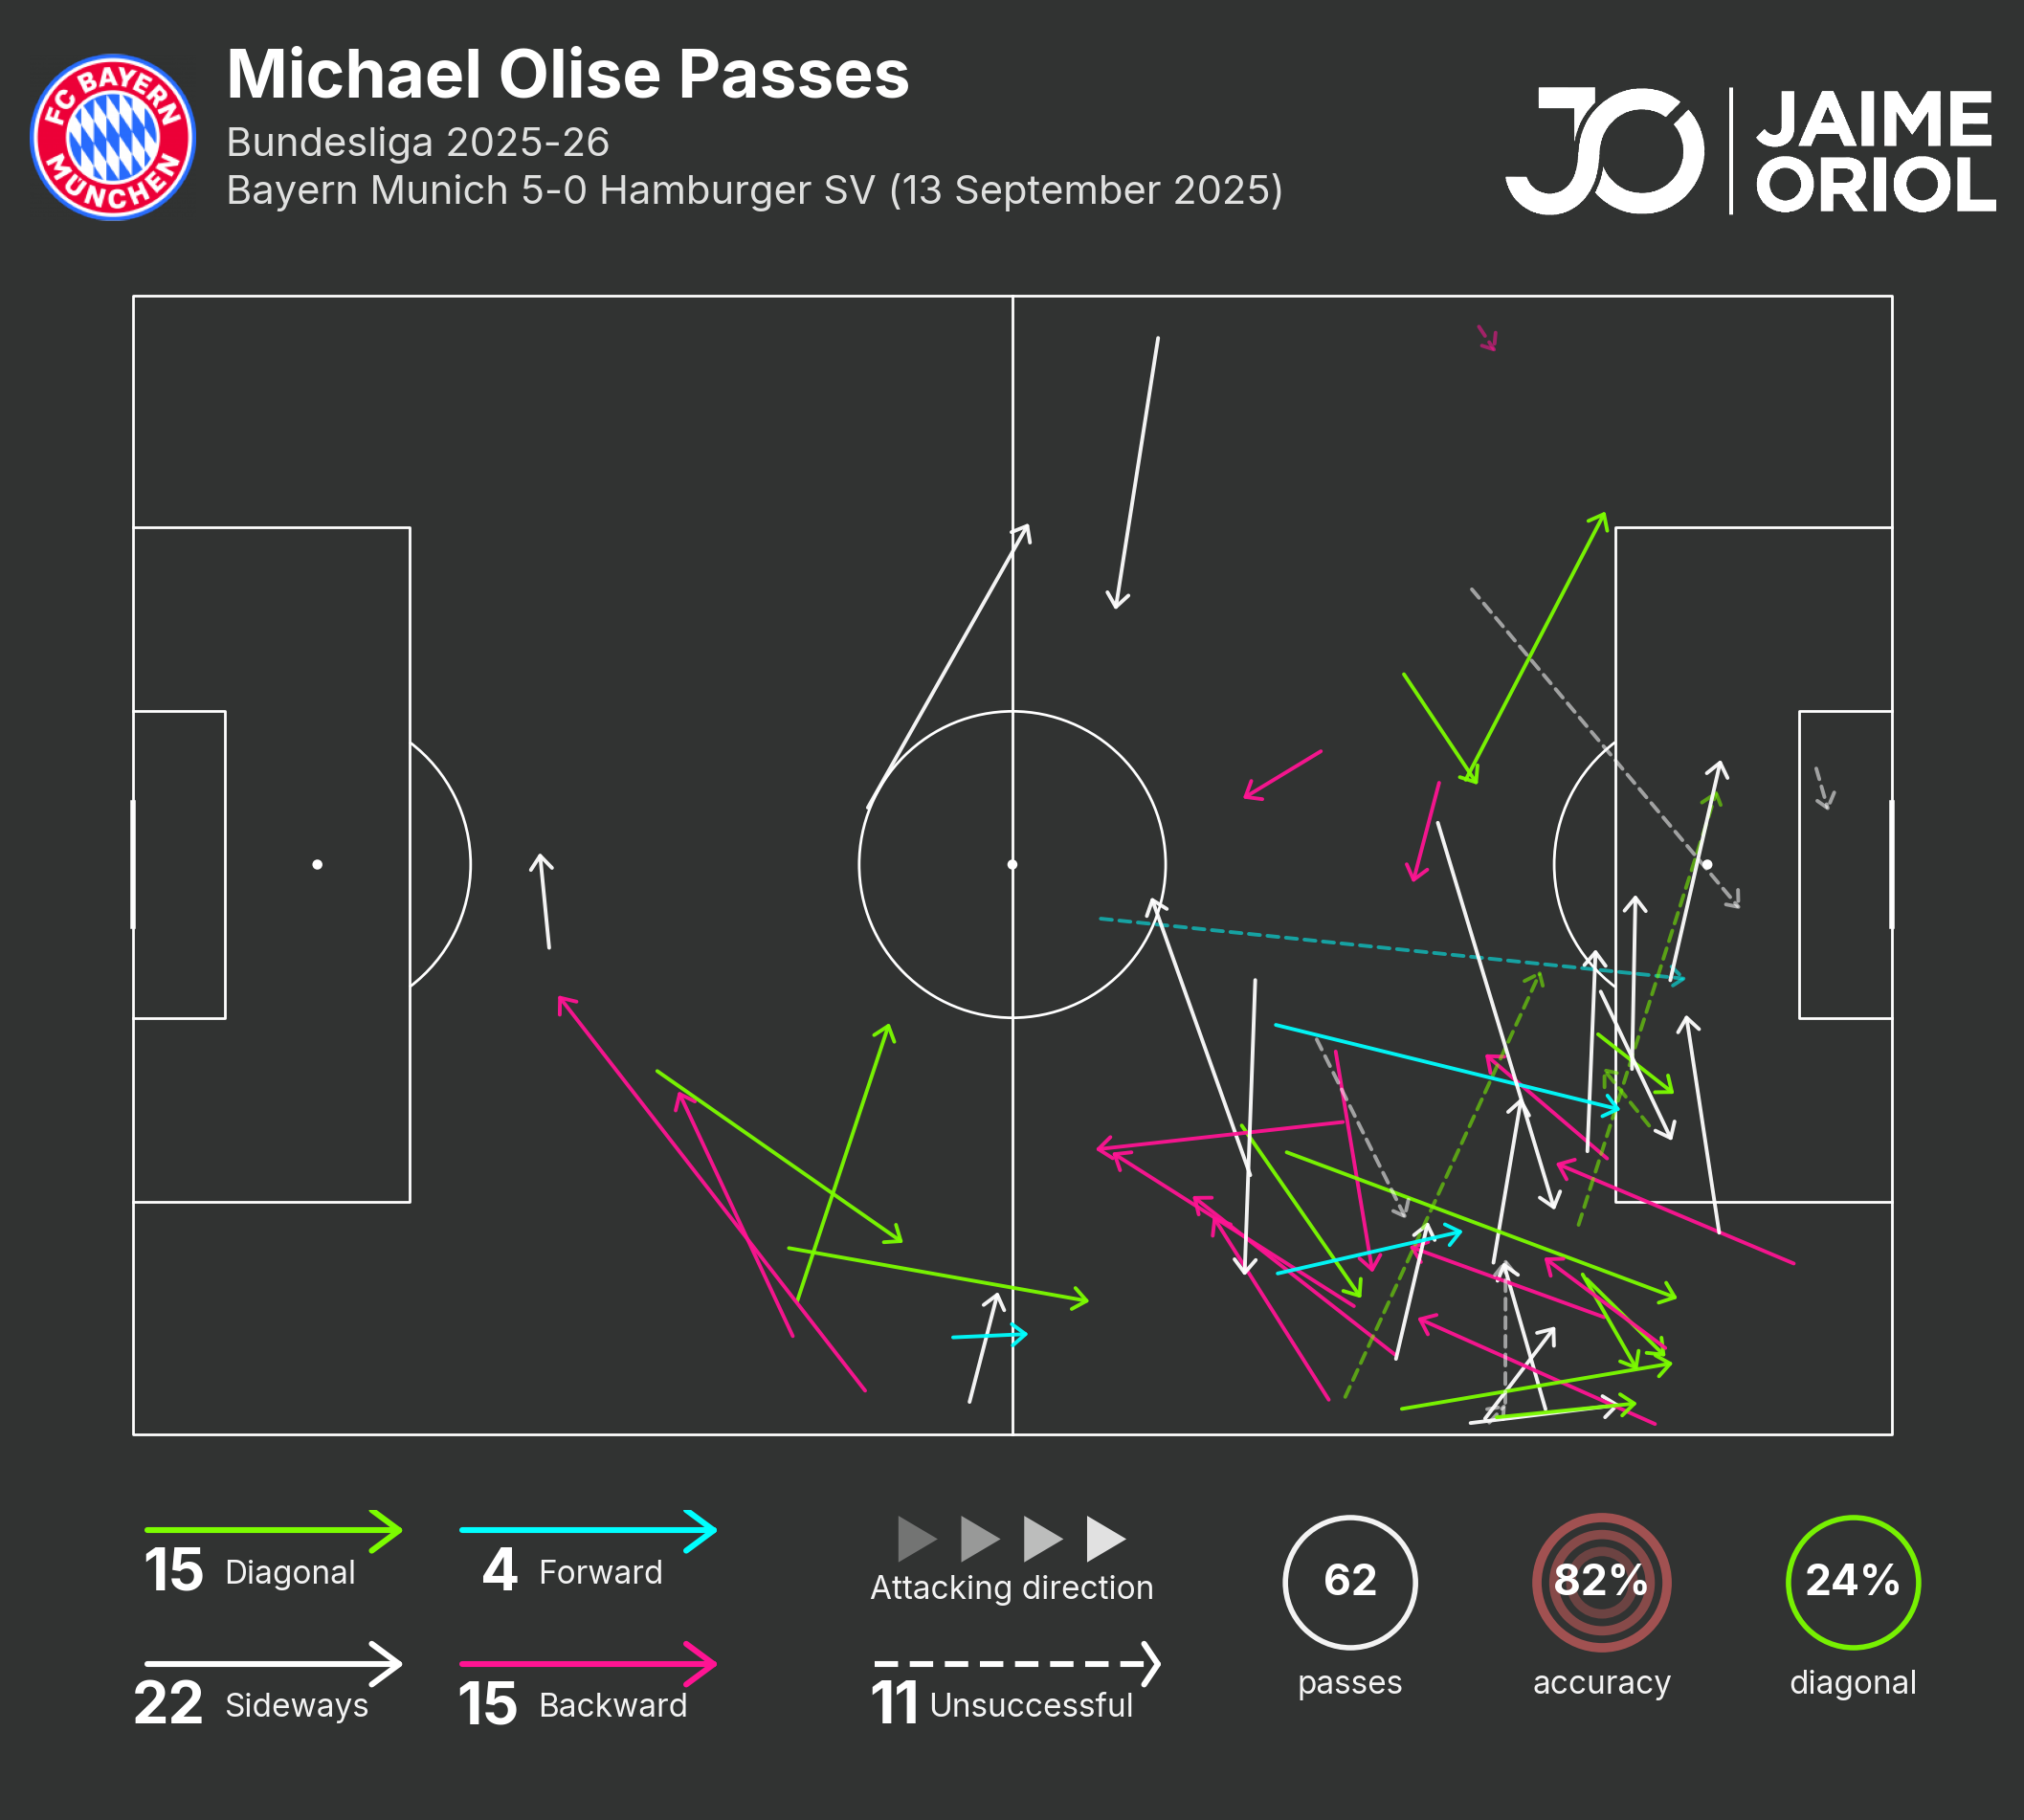
\includegraphics[width=0.74\textwidth]{Michael_Olise_Bayern_Hamburg.png}
  \caption{\textbf{Player application: Michael Olise, Bayern 5--0
  Hamburg.} Pass map coloured by DFL direction class. The per-player,
  per-opponent diagonal profile is a direct scouting output of the
  framework.}
  \label{fig:olise}
\end{figure}

% =====================================================================
\section{Applications}
\label{sec:applications}

The framework supports four concrete uses. \textbf{Match preparation:} DOS
aggregated per opponent over several matches is a map of that team's
orientation vulnerabilities --- where, and against which defenders, to
attack diagonally. \textbf{Post-match analysis:} every pass, carry,
take-on and run is annotated with DOS, defender misalignment and the
detection delay it exploited, turning ``play more diagonals'' into a
filterable, measurable behaviour. \textbf{Recruitment:} players are
profiled by how much DOS they generate and how diagonal their action and
run mix is --- a profile that, like SkillCorner's run profiles
\citep{skillcorner2024}, is stable enough to scout on. \textbf{Broadcast:}
the vision, pitch-control and DOS surfaces are visually immediate overlays
--- a defender's blind spot, lit up, with the ball arriving from the
unseen angle.

% =====================================================================
\section{Limitations and Future Work}
\label{sec:limitations}

Four limitations bound this work. \textbf{(1)} Five matches is a modest
sample; the per-event tests are well powered, but per-team and per-player
aggregates should be read as indicative. \textbf{(2)} Off-ball runs enter
through a deliberately lightweight detector; a learned run-detection
front-end, of the kind already productised by SkillCorner
\citep{skillcorner2024} and Stats Perform \citep{optavision2025}, would
let DOS score every run in a match --- the natural next step, since the
DOS engine is already action-independent. \textbf{(3)} The
orientation-aware pitch-control function is validated indirectly, through
DOS; a direct comparison of pass-completion AUC against a standard
pitch-control model \citep{spearman2017,anzer2022} is outstanding.
\textbf{(4)} DOS measures visual asymmetry; D-Def measures structural
disruption. The two are complementary rather than redundant, and
characterising that relationship deserves its own study.

% =====================================================================
\section{Conclusion}
\label{sec:conclusion}

Diagonality was football's most discussed unquantified idea. We did two
things with it. We \emph{tested} it: on five Bundesliga matches the
article's claims hold --- the diagonal is the optimum of the
progression--safety trade-off, it disrupts the defensive block on the axis
a vertical pass leaves intact, and it hands the receiver a body already
turned toward goal. And we \emph{operationalised} it: the Diagonal
Opportunity Surface turns the validated theory into an actionable,
real-time, per-opponent map of where a diagonal delivery breaks a defender
who cannot see it. In Spielverlagerung's words, ``horizontal keeps you
safe; vertical gets you killed or crowned; \dots\ diagonal lets you decide
while still in motion'' \citep{spielverlagerung2025}. We have turned that
sentence into a number on a pitch.

% =====================================================================
\bibliographystyle{plainnat}
\bibliography{references}

\end{document}
